\documentclass[11pt,a4paper]{article}

\usepackage[utf8]{inputenc}
\usepackage[margin=1in]{geometry}
\usepackage{graphicx}
\usepackage{booktabs}
\usepackage{amsmath}
\usepackage{amssymb}
\usepackage{hyperref}
\usepackage{xcolor}
\usepackage{listings}
\usepackage{float}
\usepackage{caption}
\usepackage{enumitem}
\usepackage{fancyhdr}

\hypersetup{
    colorlinks=true,
    linkcolor=blue,
    urlcolor=blue,
    citecolor=blue
}

\pagestyle{fancy}
\fancyhf{}
\rhead{Transaction Dataset Analysis}
\lhead{\thepage}
\cfoot{}

\title{\textbf{Transaction Dataset Analysis Report} \\
\large EDA, Segmentation, Forecasting, and Clustering}
\author{Ruslan Sadigov}
\date{April 2026}

\begin{document}

\maketitle

\begin{abstract}
This report presents a comprehensive analysis of a 1{,}000{,}000-row transaction dataset spanning April 2022 to December 2024. The analysis covers data cleaning, exploratory data analysis, customer segmentation via Recency-Frequency (RF) analysis, organization co-occurrence patterns via FP-Growth, time-series forecasting with SARIMA, Auto ARIMA, and Chronos foundation model, and hierarchical clustering of organizations. Key findings include the overwhelming dominance of a single organization (Org~49 with 62\% of transactions), strong weekly seasonality in transaction volume, and the superior performance of the Chronos foundation model over classical time-series approaches (MAPE 25.15\% vs 32.98\% for manual SARIMA).
\end{abstract}

\tableofcontents
\newpage

\section{Introduction}

The dataset consists of transactions between persons and organizations. Each transaction is initiated by a person with an organization, which the organization either acknowledges or refuses. This analysis aims to uncover behavioral patterns, segment customers, forecast future volume, and identify organizational clusters based on operational characteristics.

\subsection{Dataset Overview}

\begin{table}[H]
\centering
\begin{tabular}{ll}
\toprule
\textbf{Attribute} & \textbf{Value} \\
\midrule
Total rows & 1{,}000{,}000 \\
File & \texttt{data/transactions.csv} \\
Lookup file & \texttt{data/operation\_statuses.csv} \\
Date range & April 14, 2022 -- December 31, 2024 \\
Unique organizations & 95 \\
Unique persons & 235{,}506 \\
Unique card numbers & 323{,}393 \\
\bottomrule
\end{tabular}
\caption{Dataset basic statistics}
\end{table}

\subsection{Schema}

\begin{table}[H]
\centering
\begin{tabular}{lll}
\toprule
\textbf{Column} & \textbf{Type} & \textbf{Description} \\
\midrule
Id & Integer & Transaction ID (non-unique, recycled) \\
OrgId & Integer & Organization identifier \\
TransactionTypeId & Integer & Type of transaction (1 or 2) \\
Transaction\_Date & Datetime & Timestamp of the transaction \\
OperationStatusId & Integer & Status code (10, 20, or 30) \\
CardlNumber & String & Card-like identifier (nullable) \\
PersonId & Integer & Person identifier \\
\bottomrule
\end{tabular}
\caption{Dataset schema}
\end{table}

The \texttt{OperationStatusId} refers to a lookup table with three defined statuses: 10 (Acknowledged), 20 (Refused), and 30 (Initiated). Only statuses 10 and 20 are observed in the data.

\section{Data Loading and Cleaning}

\subsection{Initial Processing}

The raw CSV was loaded and merged with the \texttt{OperationStatuses} lookup table to enrich the dataset with human-readable status names. The \texttt{Transaction\_Date} column was converted from string format to datetime objects to enable temporal analysis.

\subsection{Null Value Handling}

Only one column contained null values:
\begin{itemize}
    \item \texttt{CardlNumber}: 92{,}868 nulls (9.3\% of rows)
\end{itemize}

These were filled with the placeholder string \texttt{'No Card'} to make the absence of a card explicit and to prevent issues with groupby operations that silently drop NaN values.

\subsection{Duplicate ID Investigation}

An unexpected finding was that 23{,}845 transaction IDs appeared more than once. Detailed investigation revealed:

\begin{itemize}
    \item Every duplicate ID appears exactly \textbf{twice}, never three or more times
    \item The \texttt{PersonId} is \textbf{always different} between duplicate records
    \item \texttt{OrgId} differs in 14{,}725 cases and matches in 9{,}120 cases
    \item The time gap between paired transactions has a median of \textbf{240 days}
\end{itemize}

\paragraph{Conclusion.} The \texttt{Id} column is \textbf{not a reliable unique identifier}. It appears to be recycled over time, so the same ID genuinely refers to two unrelated transactions. Both records are retained as legitimate separate transactions.

\subsection{Feature Engineering}

Additional temporal features were extracted from \texttt{Transaction\_Date}:
\begin{itemize}
    \item \texttt{Year}, \texttt{Month}, \texttt{Day}
    \item \texttt{Hour}
    \item \texttt{DayOfWeek}
\end{itemize}

These support later time-series analysis and potential ML feature inputs.

\section{Exploratory Data Analysis}

\subsection{Monthly Transaction Volume}

\begin{figure}[H]
    \centering
    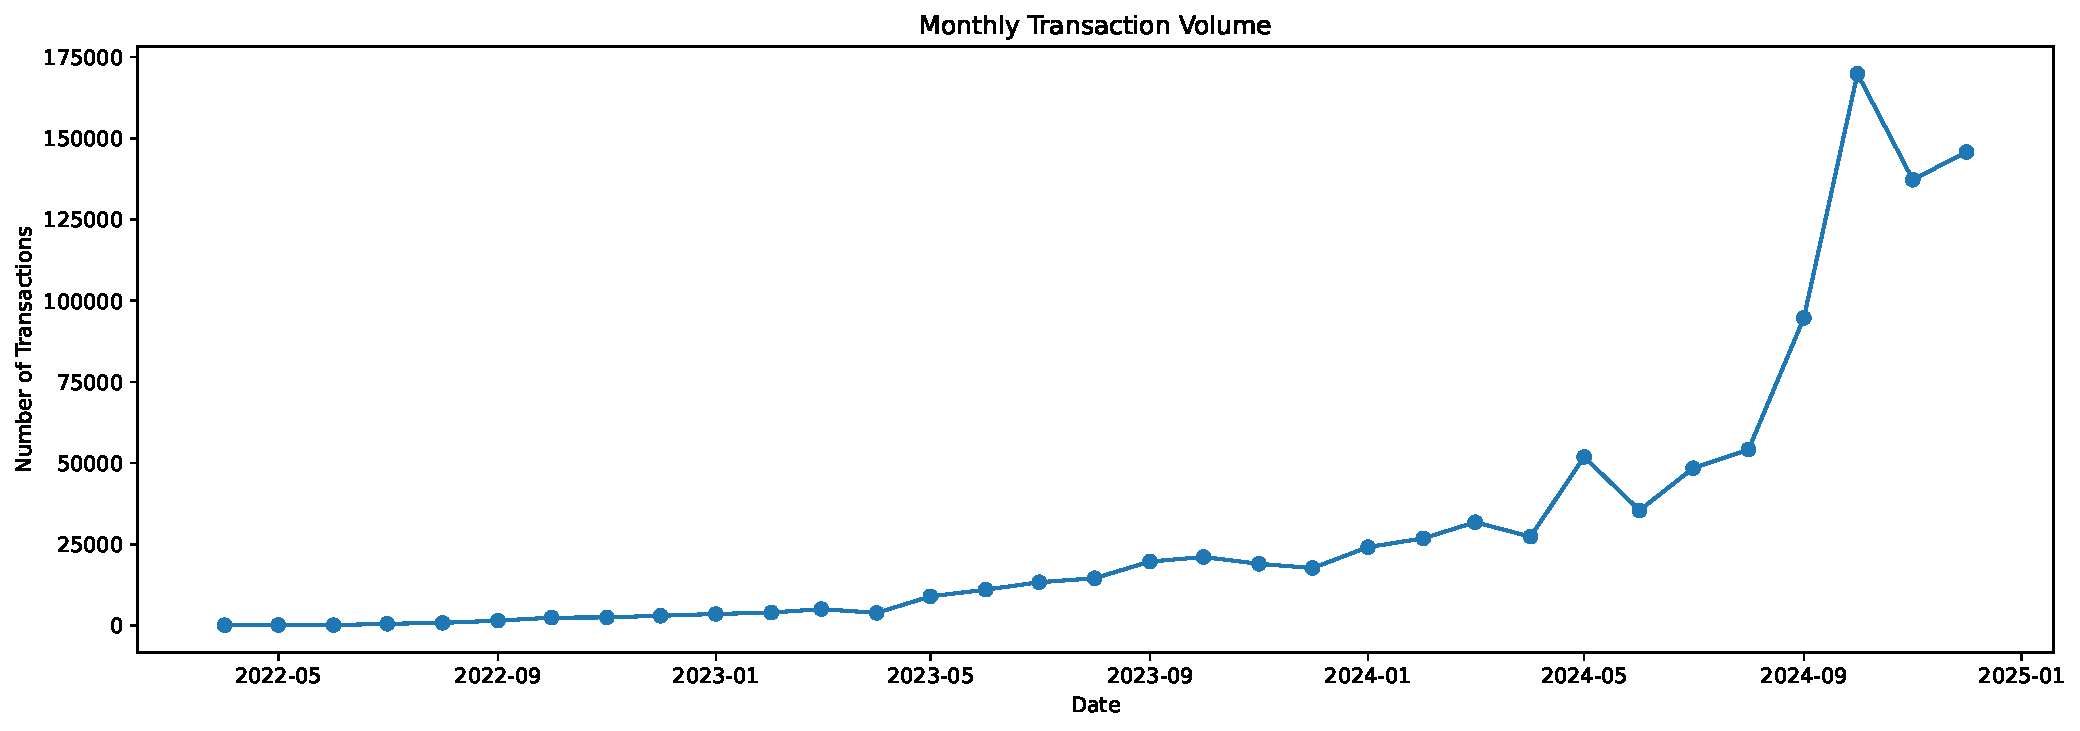
\includegraphics[width=\textwidth]{assets/monthly_volume.pdf}
    \caption{Monthly transaction volume from April 2022 to December 2024, showing strong upward growth with a notable spike in May 2024.}
\end{figure}

The monthly volume chart reveals a strong upward trend:
\begin{itemize}
    \item 2022: 10{,}927 transactions (partial year from April)
    \item 2023: 141{,}565 transactions
    \item 2024: 847{,}508 transactions
\end{itemize}

The growth is approximately 6$\times$ from 2023 to 2024. A notable spike occurs in May 2024 (51{,}888 transactions) followed by a drop in June (35{,}434), and a peak in October 2024 (169{,}877 transactions).

\subsection{Spike Investigation: April--June 2024}

Per-month breakdown of the transition period:

\begin{table}[H]
\centering
\begin{tabular}{lrrr}
\toprule
\textbf{Metric} & \textbf{April 2024} & \textbf{May 2024} & \textbf{June 2024} \\
\midrule
Total transactions & 27{,}325 & 51{,}888 & 35{,}434 \\
Unique organizations & 38 & 41 & 39 \\
Type 1 transactions & 8{,}346 & 9{,}908 & 6{,}197 \\
Type 2 transactions & 18{,}979 & 41{,}980 & 29{,}237 \\
Refused (status 20) & 9{,}108 & 597 & 0 \\
Top org (Org 49) & 15{,}794 & 37{,}512 & 25{,}998 \\
\bottomrule
\end{tabular}
\caption{Comparison of April, May, and June 2024}
\end{table}

Investigation showed that \textbf{Org~49 alone was responsible for 72\% of May 2024 transactions}. The spike was not due to new organizations or a widespread surge; it was driven entirely by one organization's activity.

\subsection{Org 49 Dominance}

\begin{figure}[H]
    \centering
    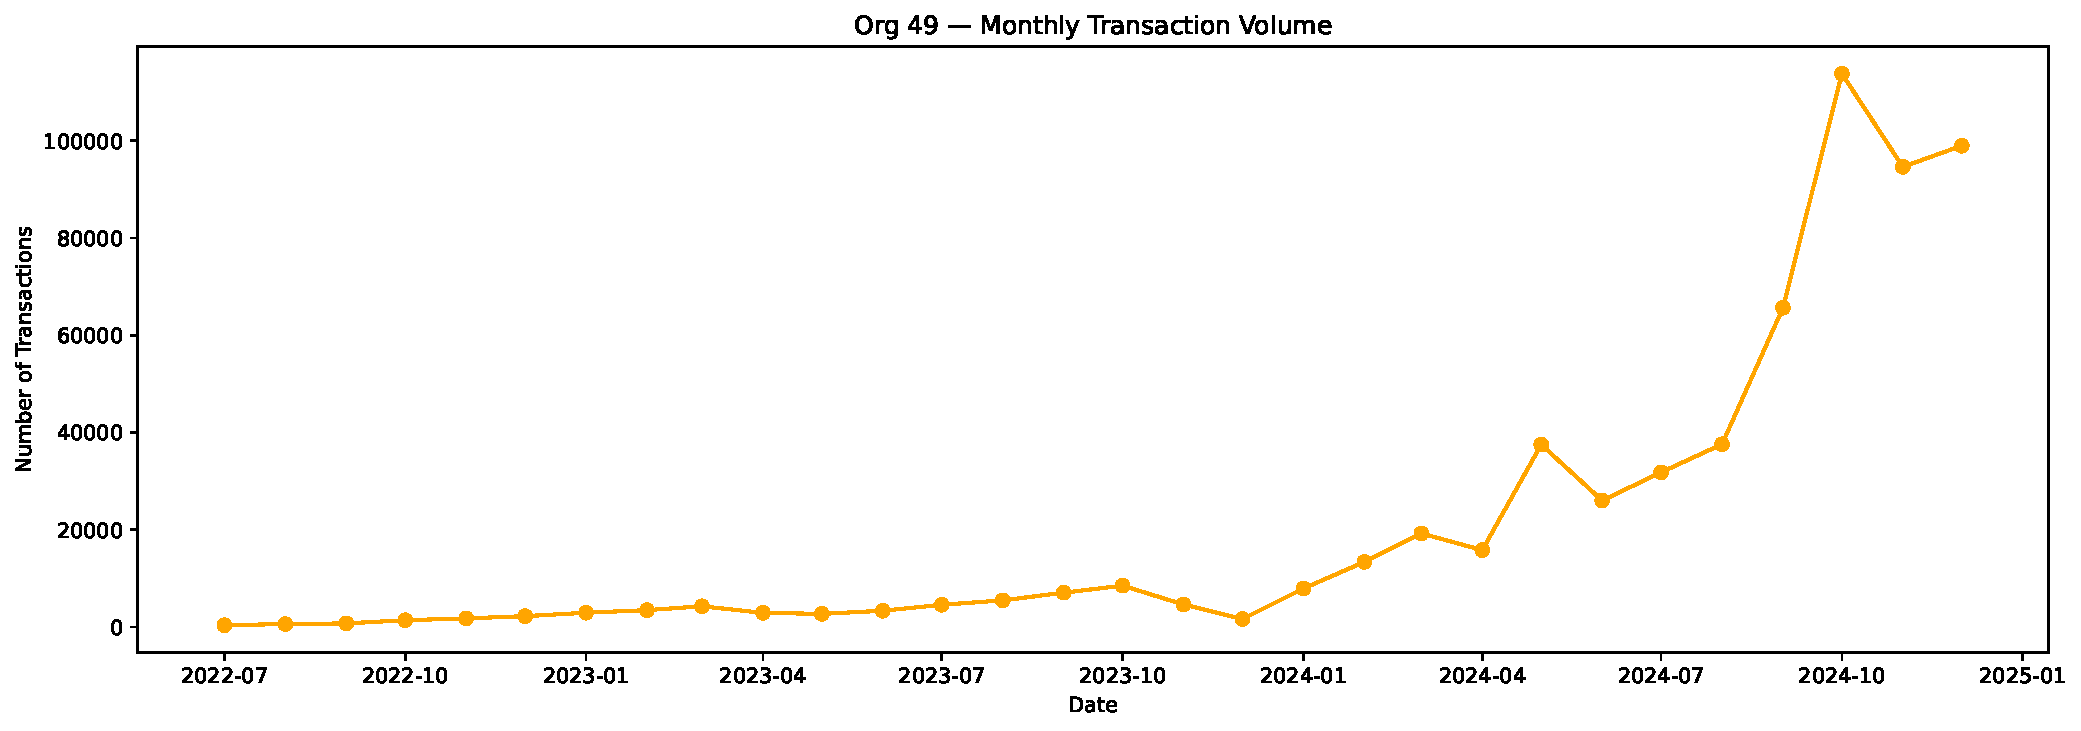
\includegraphics[width=\textwidth]{assets/org49_monthly_volume.pdf}
    \caption{Monthly transaction volume of Org 49, nearly identical in shape to the overall dataset volume, confirming its dominant influence on aggregate transaction patterns.}
\end{figure}

The monthly chart for Org~49 is nearly identical in shape to the overall dataset chart. Quantitatively:

\begin{itemize}
    \item Org 49 accounts for \textbf{620{,}445} of 1{,}000{,}000 transactions (\textbf{62.0\%})
    \item Org 49 serves \textbf{162{,}649} of 235{,}506 unique persons (\textbf{69.1\%})
\end{itemize}

This single-org dominance shapes nearly every subsequent analysis and is a recurring theme throughout this report.

\subsection{Top Organizations by Volume}

\begin{figure}[H]
    \centering
    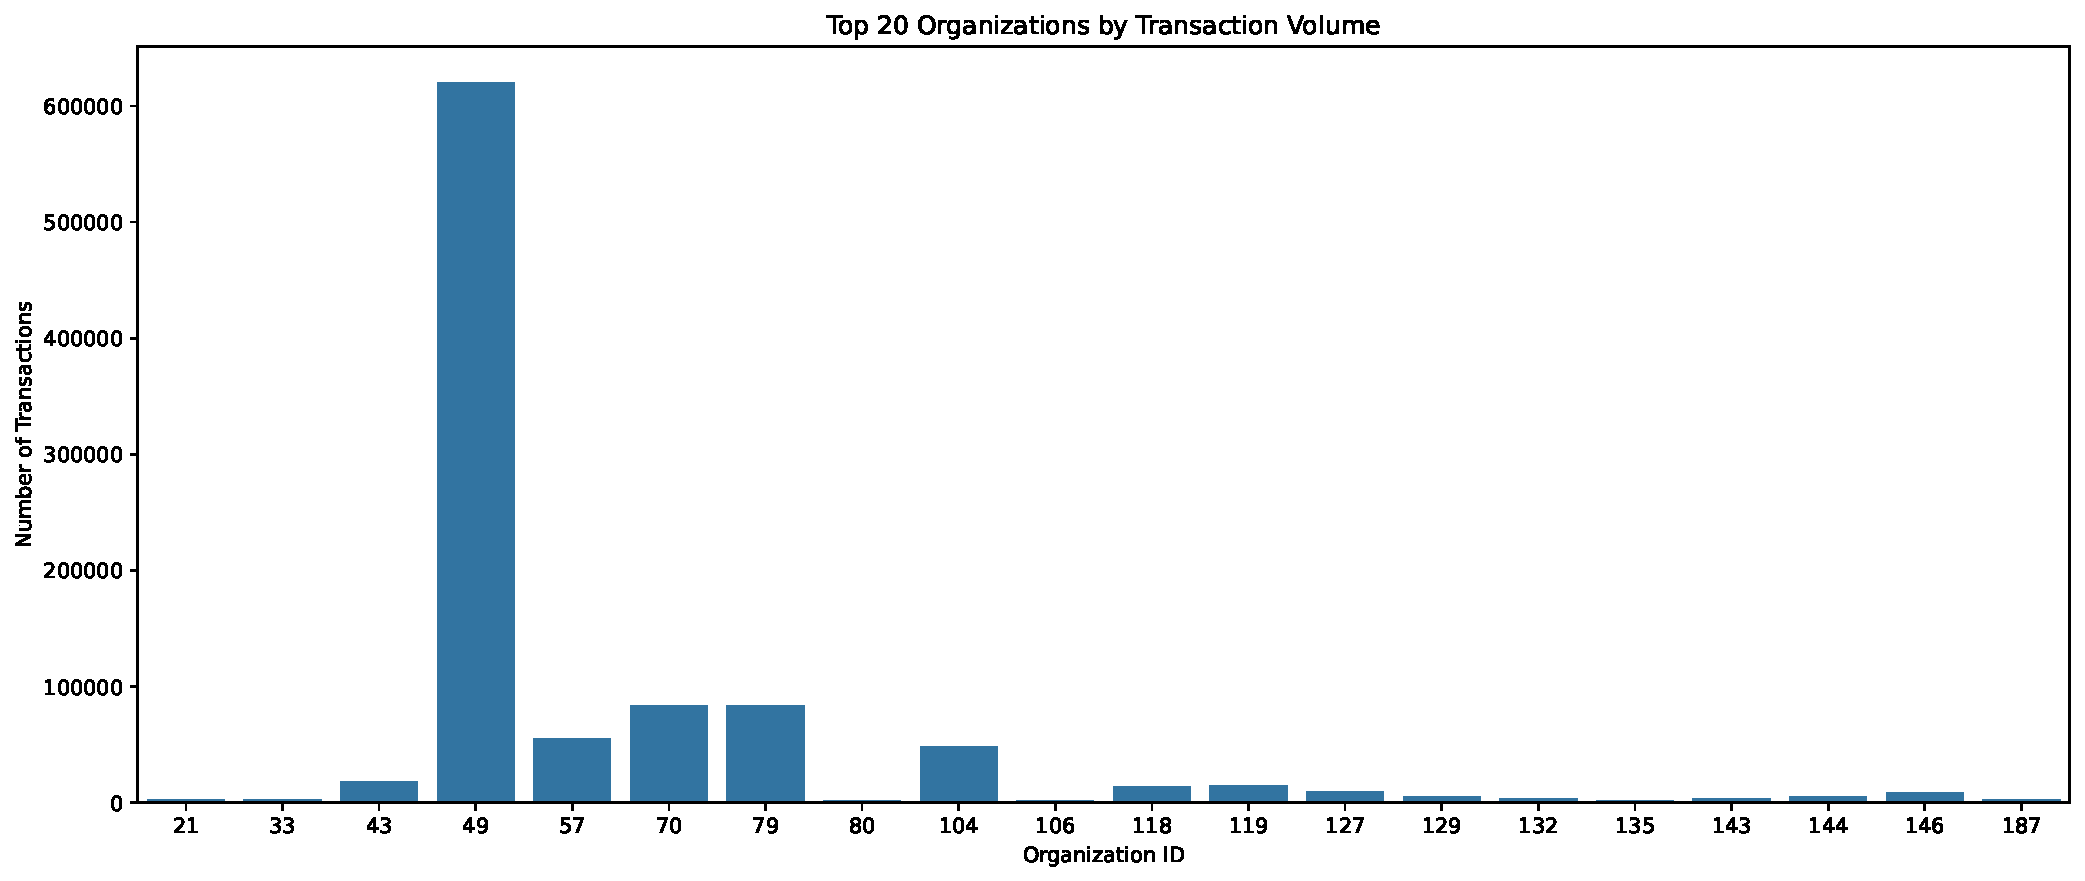
\includegraphics[width=\textwidth]{assets/top20_orgs_volume.pdf}
    \caption{Top 20 organizations by transaction volume, dominated by Org 49 which alone accounts for 62\% of all transactions.}
\end{figure}

\begin{figure}[H]
    \centering
    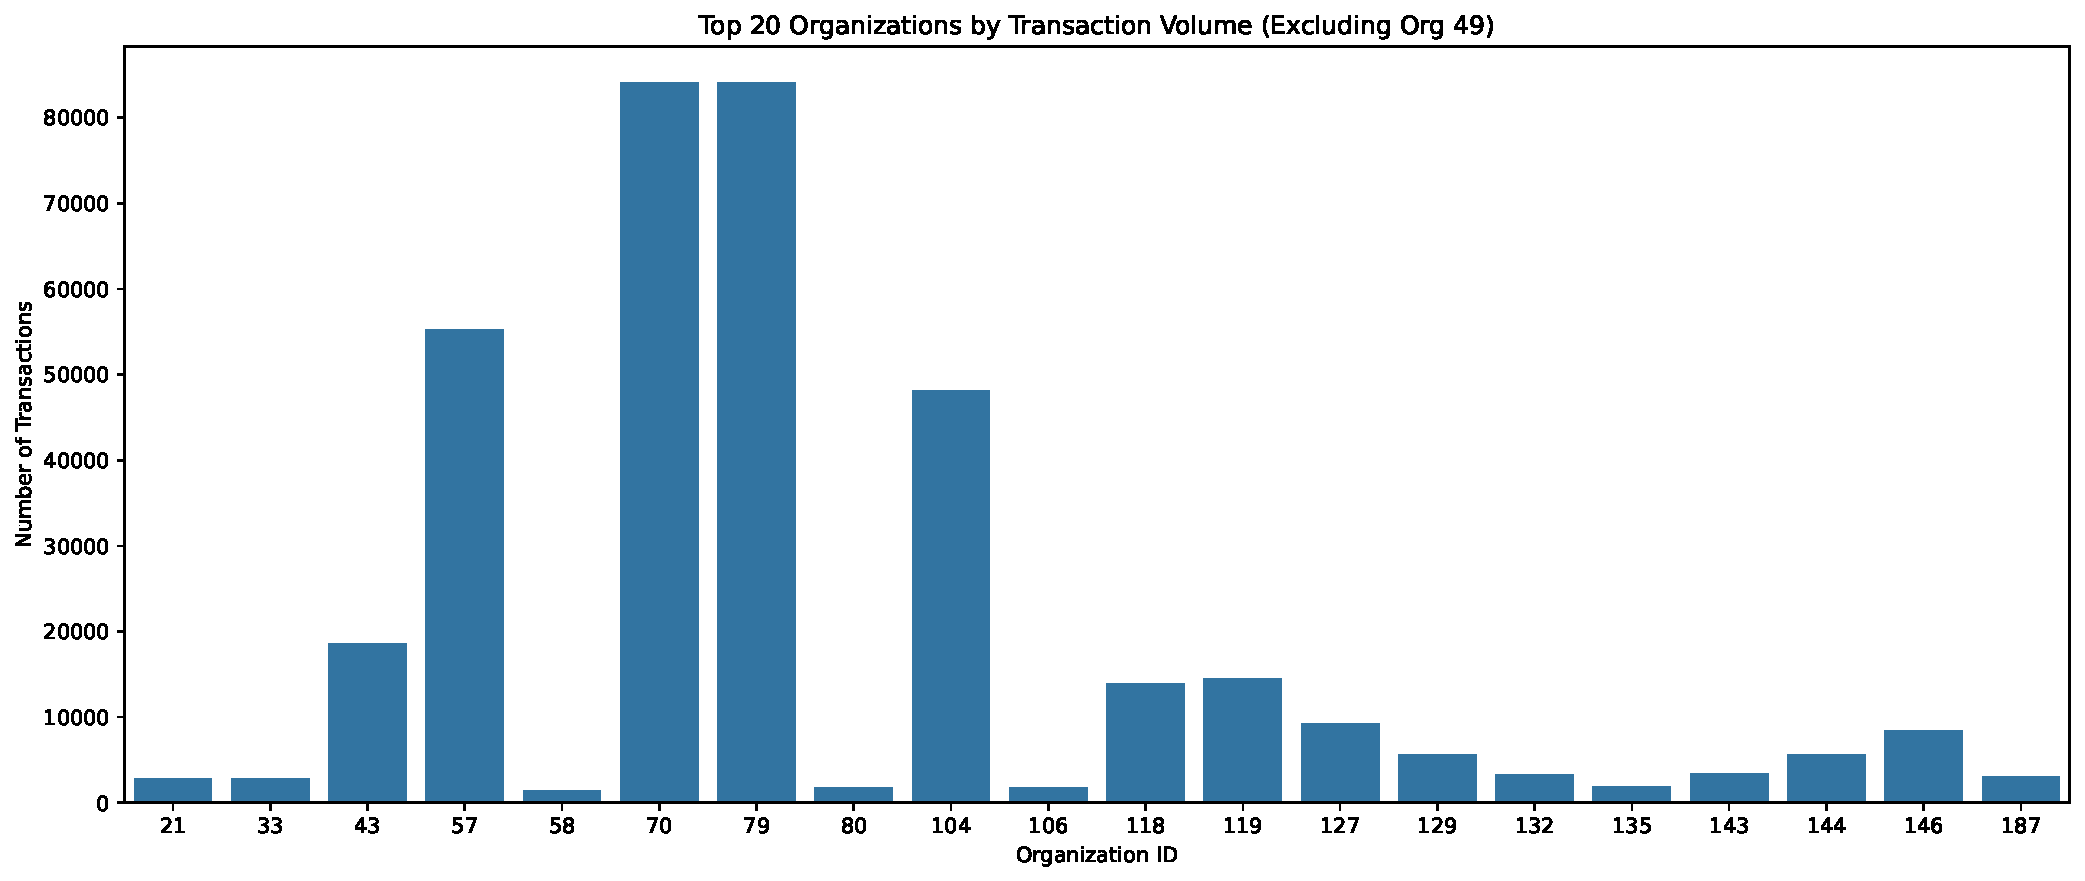
\includegraphics[width=\textwidth]{assets/top20_orgs_volume_ex49.pdf}
    \caption{Top 20 organizations by transaction volume excluding Org 49, revealing a second tier led by Orgs 70 and 79 with approximately 84{,}000 transactions each.}
\end{figure}
  
\begin{table}[H]
\centering
\begin{tabular}{rrr}
\toprule
\textbf{OrgId} & \textbf{Transactions} & \textbf{Share (\%)} \\
\midrule
49 & 620{,}445 & 62.0 \\
70 & 84{,}128 & 8.4 \\
79 & 84{,}081 & 8.4 \\
57 & 55{,}313 & 5.5 \\
104 & 48{,}129 & 4.8 \\
43 & 18{,}604 & 1.9 \\
119 & 14{,}522 & 1.5 \\
118 & 13{,}918 & 1.4 \\
\bottomrule
\end{tabular}
\caption{Top 8 organizations by transaction volume}
\end{table}

The tiered structure is clear: one dominant org, a small cluster of high-volume orgs (70, 79, 57, 104), and a long tail of smaller organizations. Notably, Orgs~70 and~79 have nearly identical transaction counts (84{,}128 vs 84{,}081), suggesting possible relationship or coordinated activity.

\section{Customer Segmentation: RF Analysis}

\subsection{Methodology}

RF analysis (Recency--Frequency) was used instead of full RFM since the dataset contains no monetary value column. For each unique person:
\begin{itemize}
    \item \textbf{Recency}: days since last transaction (reference date: 2024-12-31)
    \item \textbf{Frequency}: total number of transactions
\end{itemize}

\subsection{Scoring Approach}

Manual thresholds via \texttt{pd.cut} were used instead of percentile-based \texttt{qcut} due to the heavy skew in frequency (34.8\% of persons have exactly one transaction). Manual thresholds also provide more interpretable bucket boundaries.

\paragraph{Recency bins (days):}
\begin{itemize}[noitemsep]
    \item Score 4: 0--30 (very active)
    \item Score 3: 31--90
    \item Score 2: 91--180
    \item Score 1: 181+ (inactive)
\end{itemize}

\paragraph{Frequency bins (transaction count):}
\begin{itemize}[noitemsep]
    \item Score 1: exactly 1 (one-timer)
    \item Score 2: 2--3 (occasional)
    \item Score 3: 4--10 (regular)
    \item Score 4: 11+ (heavy user)
\end{itemize}

\subsection{Segment Assignment Logic}

\begin{table}[H]
\centering
\begin{tabular}{llll}
\toprule
\textbf{Segment} & \textbf{R Score} & \textbf{F Score} & \textbf{Interpretation} \\
\midrule
Champions & 4 & 4 & Recent and heavy users \\
Loyal & $\geq 3$ & $\geq 3$ & Active and regular \\
At Risk & $\leq 2$ & $\geq 3$ & Used to be active \\
Lost & 1 & $\leq 2$ & Inactive, low usage \\
Occasional & other & other & Casual users \\
\bottomrule
\end{tabular}
\caption{Segment assignment rules}
\end{table}

\subsection{Segment Distribution}

\begin{table}[H]
\centering
\begin{tabular}{lr}
\toprule
\textbf{Segment} & \textbf{Persons} \\
\midrule
Occasional & 120{,}364 \\
Loyal & 44{,}850 \\
Lost & 43{,}011 \\
At Risk & 17{,}691 \\
Champions & 9{,}590 \\
\midrule
\textbf{Total} & \textbf{235{,}506} \\
\bottomrule
\end{tabular}
\caption{Person counts per RF segment}
\end{table}

\begin{figure}[H]
    \centering
    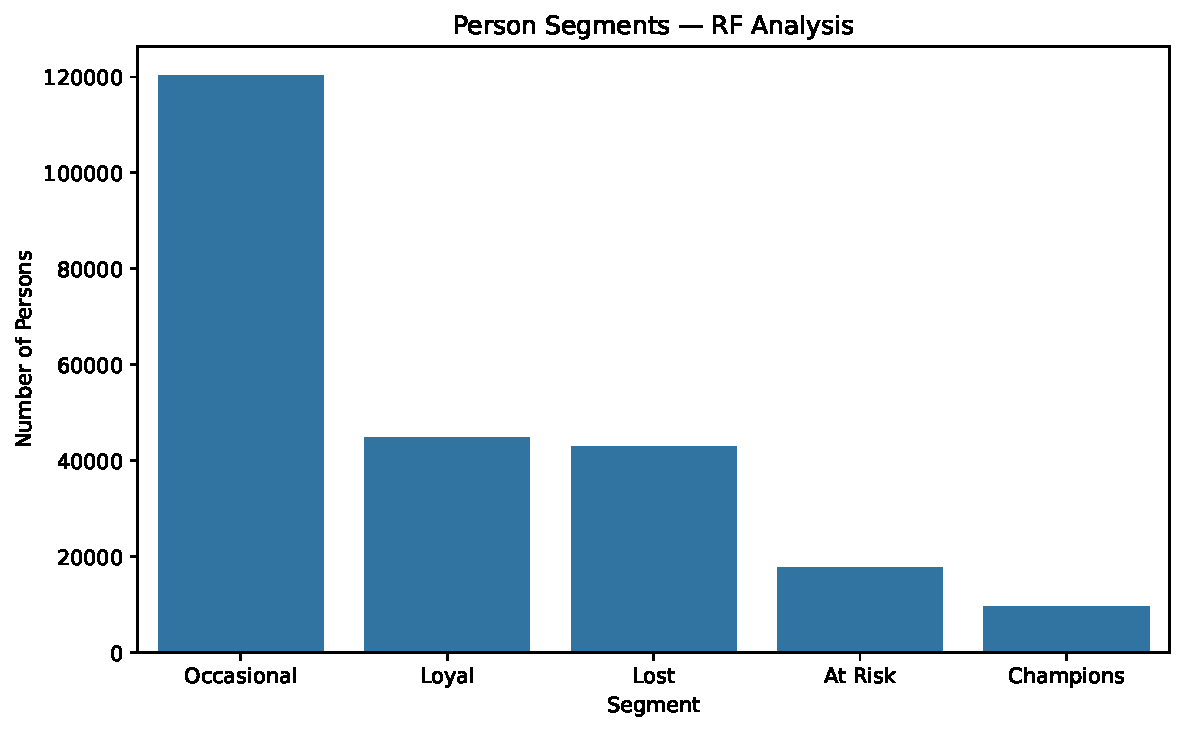
\includegraphics[width=0.8\textwidth]{assets/person_segments.pdf}
    \caption{Distribution of persons across the five RF segments, with Occasional users forming the largest group at 120{,}364 persons.}
\end{figure}

\begin{figure}[H]
    \centering
    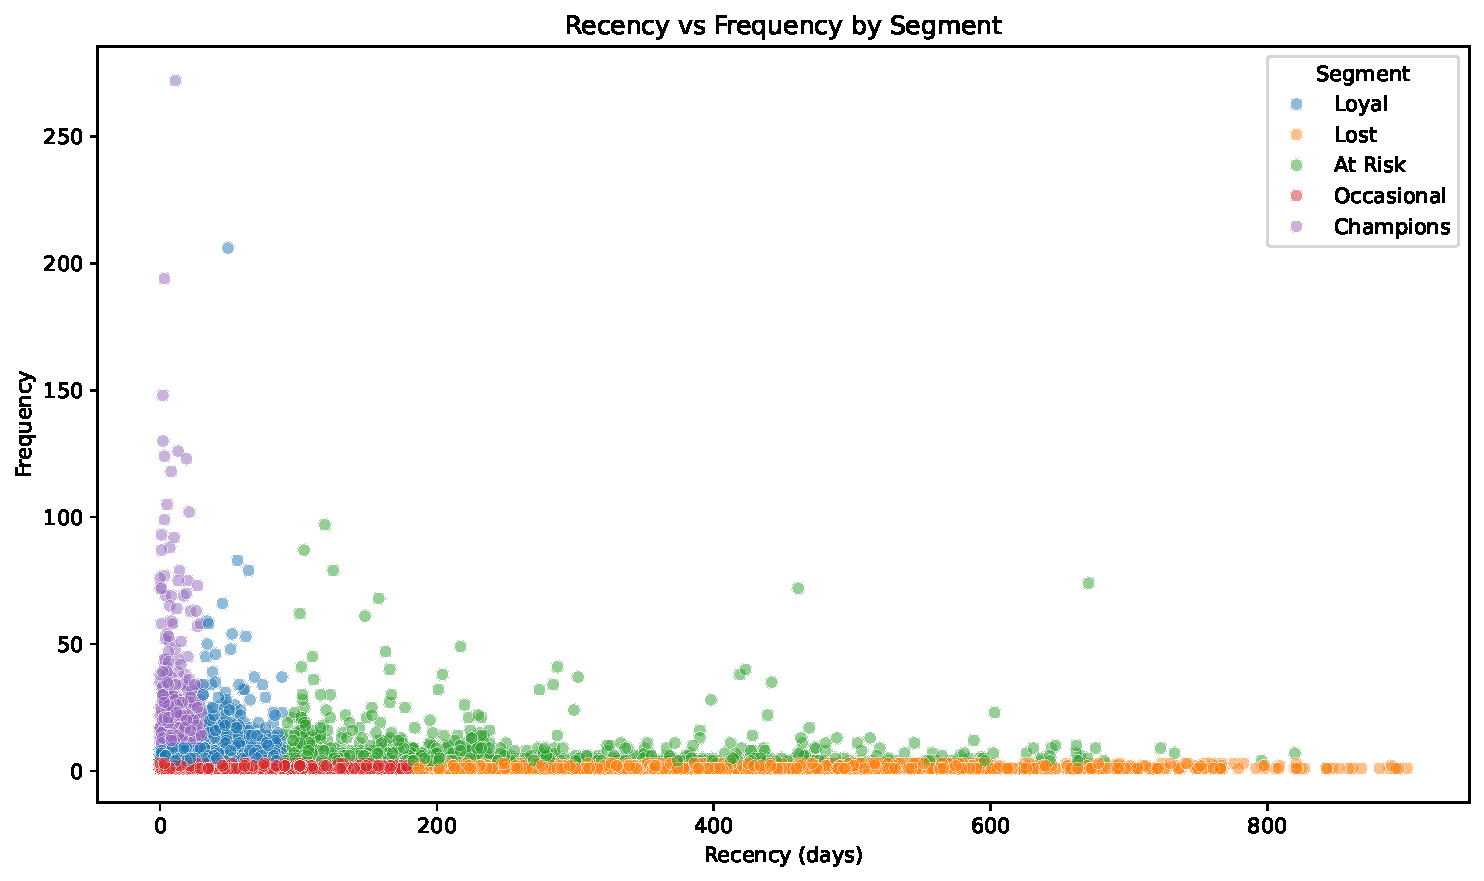
\includegraphics[width=\textwidth]{assets/recency_vs_frequency.pdf}
    \caption{Recency vs Frequency scatter plot (10{,}000 sampled persons), showing the long-tail concentration of users with low frequency and high recency.}
\end{figure}

\subsection{Segment Observations}

The scatter plot (Recency vs Frequency) shows the classic long-tail pattern of digital service usage:
\begin{itemize}
    \item Champions (purple) cluster tightly in the low-recency, high-frequency corner
    \item Loyal (blue) sit between Champions and Occasional
    \item At Risk (green) spread across medium recency with moderate-to-high frequency
    \item Lost (orange) dominate the chart with a long tail extending to high recency
    \item Occasional (red) users are densely packed at the bottom with very low frequency
\end{itemize}

Most users are one-time or rare users, and many transactions appear to be tied to specific one-off needs.

\subsection{Segment--Organization Cross Analysis}

Each bar chart below shows the top 5 organizations per segment, with the x-axis label displaying \textbf{the share of each org's total transactions} that fall within the given segment. This per-org percentage is often more revealing than raw counts because it shows how \emph{concentrated} each org's user base is in a particular behavioral group.

\begin{figure}[H]
    \centering
    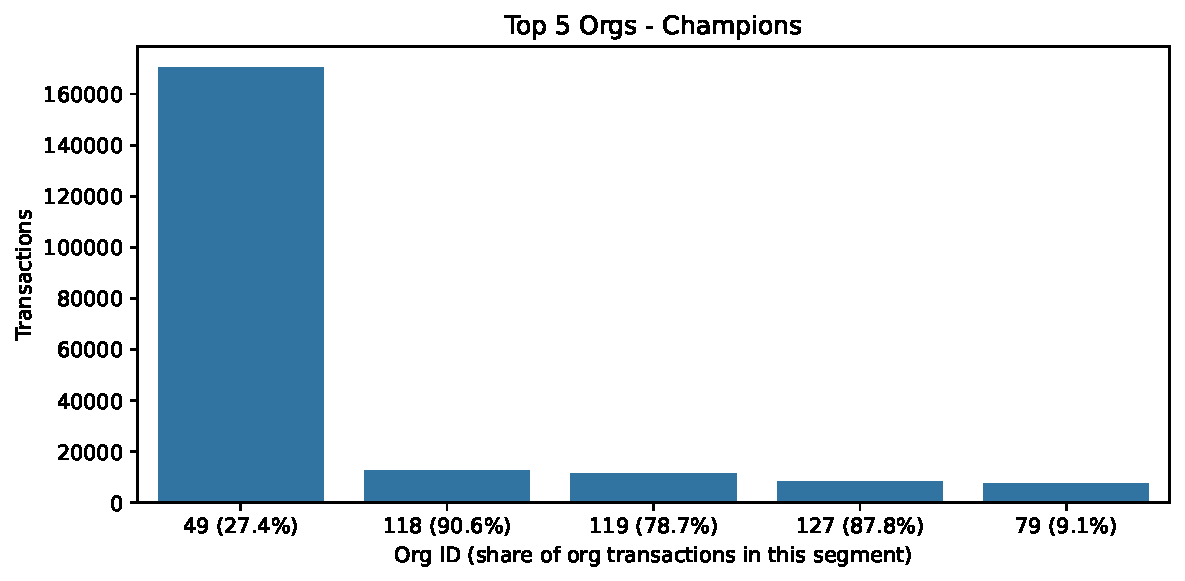
\includegraphics[width=0.8\textwidth]{assets/top5_orgs_champions.pdf}
    \caption{Top 5 organizations in the Champions segment. Orgs 118, 119, and 127 show extreme concentration of Champions users within their own bases.}
\end{figure}

\begin{figure}[H]
    \centering
    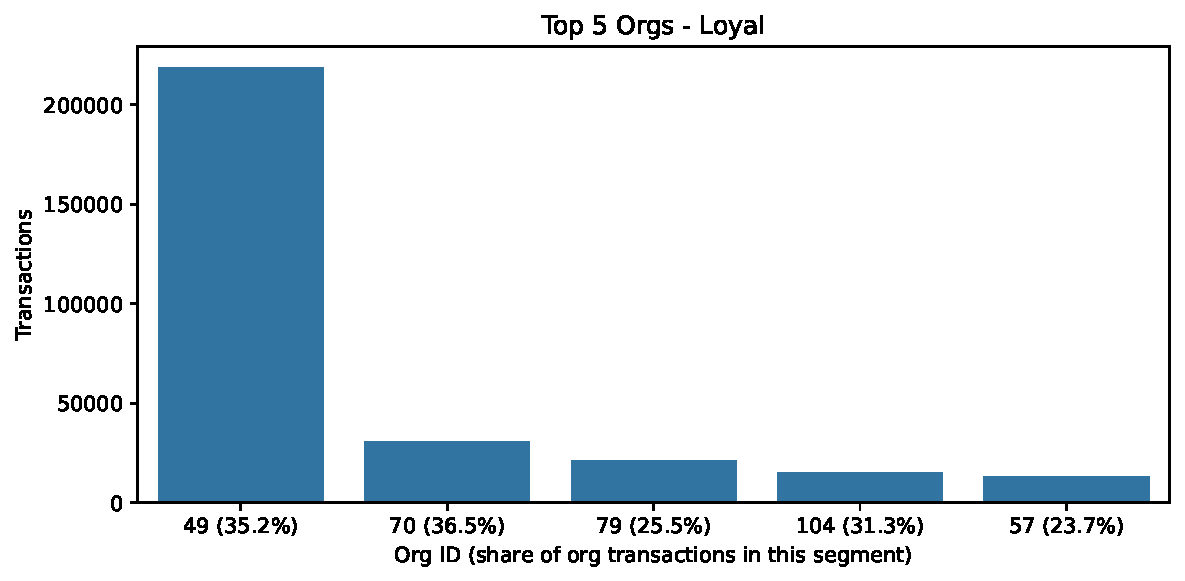
\includegraphics[width=0.8\textwidth]{assets/top5_orgs_loyal.pdf}
    \caption{Top 5 organizations in the Loyal segment, with relatively balanced Loyal shares across the major orgs.}
\end{figure}

\begin{figure}[H]
    \centering
    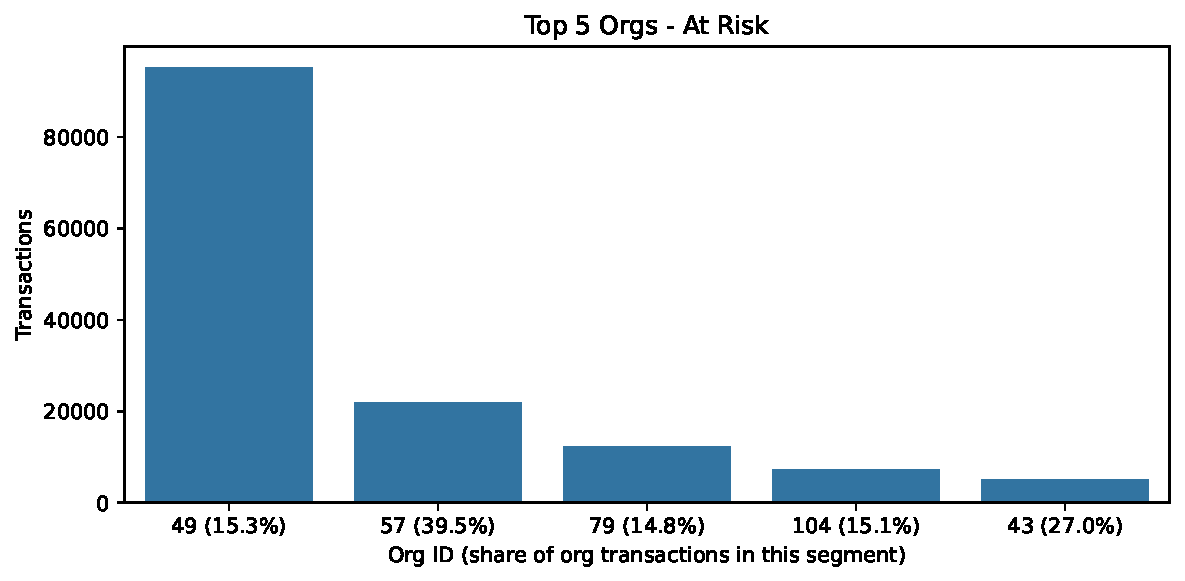
\includegraphics[width=0.8\textwidth]{assets/top5_orgs_at_risk.pdf}
    \caption{Top 5 organizations in the At Risk segment. Org 57 stands out with 39.5\% of its transactions coming from At Risk users.}
\end{figure}

\begin{figure}[H]
    \centering
    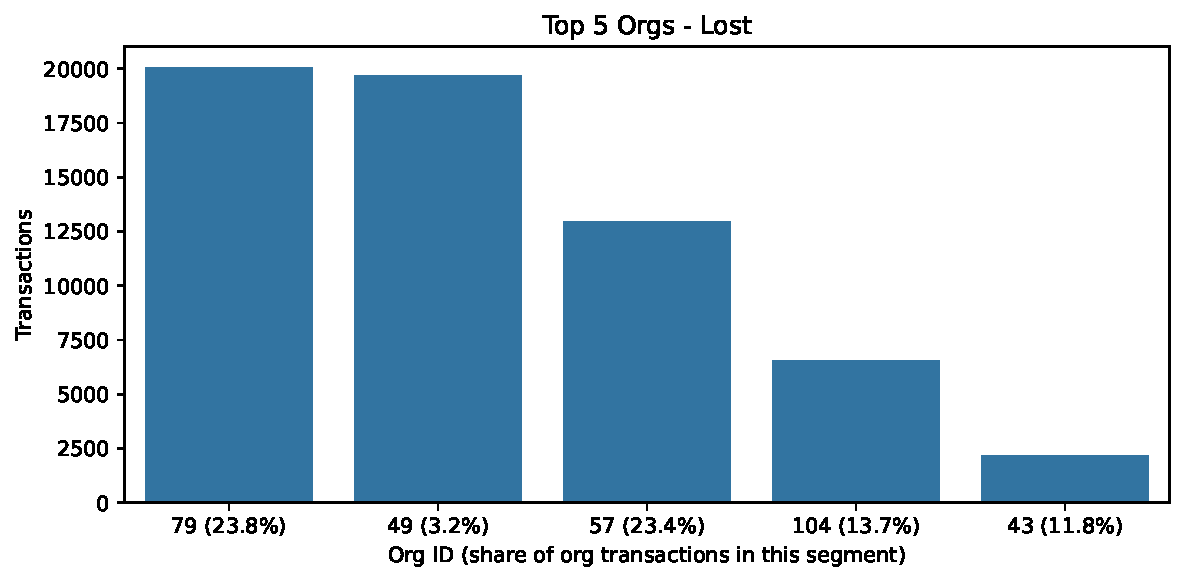
\includegraphics[width=0.8\textwidth]{assets/top5_orgs_lost.pdf}
    \caption{Top 5 organizations in the Lost segment, where Org 79 narrowly leads Org 49 (20{,}038 vs 19{,}685 transactions).}
\end{figure}

\begin{figure}[H]
    \centering
    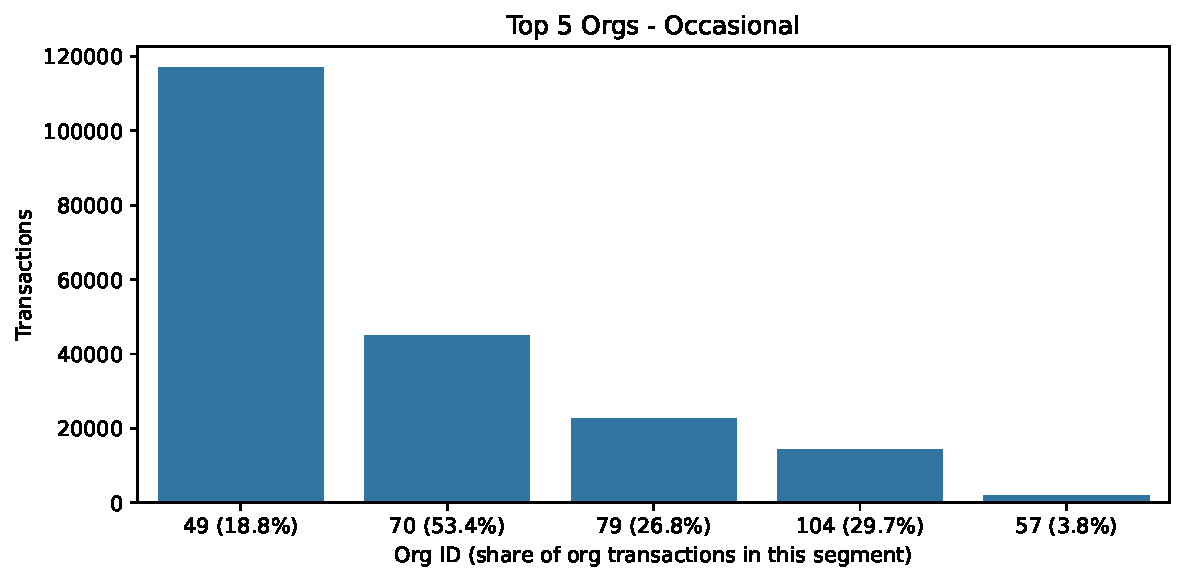
\includegraphics[width=0.8\textwidth]{assets/top5_orgs_occasional.pdf}
    \caption{Top 5 organizations in the Occasional segment. More than half of Org 70's transactions come from Occasional users.}
\end{figure}

\subsubsection{Key Observations by Segment}

\paragraph{Champions: concentration of ``loyal-base'' orgs.}
While Org~49 contributes the largest absolute count (170{,}259 transactions), the per-org share reveals three specialist organizations with remarkably concentrated user bases:
\begin{itemize}
    \item \textbf{Org 118}: 90.6\% of its transactions are from Champions (12{,}603 out of 13{,}918)
    \item \textbf{Org 127}: 87.8\% from Champions (8{,}158 out of 9{,}292)
    \item \textbf{Org 119}: 78.7\% from Champions (11{,}431 out of 14{,}522)
\end{itemize}
These three mid-size orgs are almost entirely served by recent, heavy users, indicating a dedicated, high-engagement user base. In contrast Org~49 has only 27.4\% of its transactions in Champions, and Org~79 only 9.1\%. This suggests Orgs~118, 119, and 127 operate in niches that attract consistent, repeat engagement.

\paragraph{Loyal: balanced across major orgs.}
The Loyal shares are relatively uniform across the top orgs (23.7\%--36.5\%), with Org~70 slightly leading at 36.5\%. No single org disproportionately dominates the Loyal segment, indicating that the Loyal user base is spread across multiple organizations.

\paragraph{At Risk: warning sign for Org 57.}
\textbf{Org 57 has 39.5\% of its transactions from At Risk users}, by far the highest At Risk share of any major org and 2.6$\times$ higher than the dataset-wide At Risk share. Org~43 also shows elevated At Risk concentration at 27.0\%. These percentages indicate these orgs have a growing cohort of once-active users fading away, which may warrant a retention review. For context, Org~49's At Risk share is only 15.3\%.

\paragraph{Lost: Org 79 has high churn.}
Org~79 leads both in absolute count (20{,}038) and has 23.8\% of its transactions from Lost users. Org~57 mirrors this with a 23.4\% Lost share. In contrast, \textbf{Org 49's Lost share is only 3.2\%}, the best retention metric among all major orgs, suggesting its user base remains consistently active rather than drifting away.

\paragraph{Occasional: Org 70 is dominated by casual users.}
\textbf{Over half (53.4\%) of Org 70's transactions come from Occasional users.} This is the single highest within-org share observed across any segment-org pairing and tells a clear story: despite Org~70 ranking second in total volume, its user base is overwhelmingly casual rather than devoted. Org~104 (29.7\%) and Org~79 (26.8\%) also show substantial Occasional presence. Org~49 sits at a moderate 18.8\%.

\subsubsection{Cross-Segment Summary}

Combining these observations yields distinct organizational personas:
\begin{itemize}
    \item \textbf{Deep-engagement niche orgs:} 118, 127, 119, small volume but overwhelmingly served by Champions.
    \item \textbf{Churn-risk orgs:} 57 (39.5\% At Risk) and 79 (23.8\% Lost), showing user attrition patterns.
    \item \textbf{Casual-traffic org:} 70, with 53.4\% Occasional, low stickiness despite high volume.
    \item \textbf{Healthy retention leader:} 49, with only 3.2\% Lost, suggesting strong user retention at scale.
\end{itemize}

Org~49 remains the \#1 org in every segment except Lost (where Org~79 narrowly leads, 20{,}038 vs 19{,}685), and Org~70 is notably absent from the Champions top 5 despite being the second-largest org overall, consistent with its Occasional-heavy user base.

\section{Organization Co-occurrence Analysis}

\subsection{Motivation}

Inspired by market basket analysis, this section asks: \textit{which organizations tend to share the same users?} Each person's unique set of organizations forms a ``basket.'' The FP-Growth algorithm (more efficient than Apriori) was used to find frequent itemsets and generate association rules.

\subsection{Data Preparation}

For each person, a basket was constructed containing the unique organizations they had transacted with:
\begin{itemize}
    \item Transaction counts are intentionally ignored; each org appears once per person's basket
    \item All 95 organizations including Org 49 are included (excluding it was tested but removed meaningful patterns entirely)
    \item A total of 235{,}506 baskets were analyzed
\end{itemize}

\subsection{Frequent Itemsets}

With a minimum support of 1\%, the following itemsets were identified (top items shown):

\begin{table}[H]
\centering
\begin{tabular}{lrc}
\toprule
\textbf{Itemset} & \textbf{Support} & \textbf{Length} \\
\midrule
\{49\} & 0.691 & 1 \\
\{70\} & 0.296 & 1 \\
\{49, 70\} & 0.244 & 2 \\
\{79\} & 0.232 & 1 \\
\{104\} & 0.111 & 1 \\
\{49, 79\} & 0.089 & 2 \\
\{57\} & 0.071 & 1 \\
\{49, 104\} & 0.038 & 2 \\
\{49, 70, 79\} & 0.025 & 3 \\
\{49, 43\} & 0.023 & 2 \\
\{57, 79\} & 0.021 & 2 \\
\bottomrule
\end{tabular}
\caption{Top frequent itemsets (support $\geq$ 1\%)}
\end{table}

\subsection{Association Rules}

With a minimum confidence threshold of 0.3, 14 rules were generated. Key rules ranked by lift:

\begin{table}[H]
\centering
\footnotesize
\begin{tabular}{llrrrr}
\toprule
\textbf{Antecedent} & \textbf{Consequent} & \textbf{Support} & \textbf{Confidence} & \textbf{Lift} \\
\midrule
\{57, 49\} & \{79\} & 0.010 & 0.377 & \textbf{1.625} \\
\{43\} & \{79\} & 0.012 & 0.340 & \textbf{1.466} \\
\{104, 49\} & \{79\} & 0.012 & 0.321 & 1.382 \\
\{104, 70\} & \{49\} & 0.010 & 0.858 & 1.242 \\
\{70, 79\} & \{49\} & 0.025 & 0.850 & 1.231 \\
\{146\} & \{49\} & 0.013 & 0.841 & 1.217 \\
\{70\} & \{49\} & 0.244 & 0.823 & 1.192 \\
\{43\} & \{49\} & 0.023 & 0.650 & 0.941 \\
\{79\} & \{49\} & 0.089 & 0.383 & 0.554 \\
\bottomrule
\end{tabular}
\caption{Key association rules (selected)}
\end{table}

\begin{figure}[H]
    \centering
    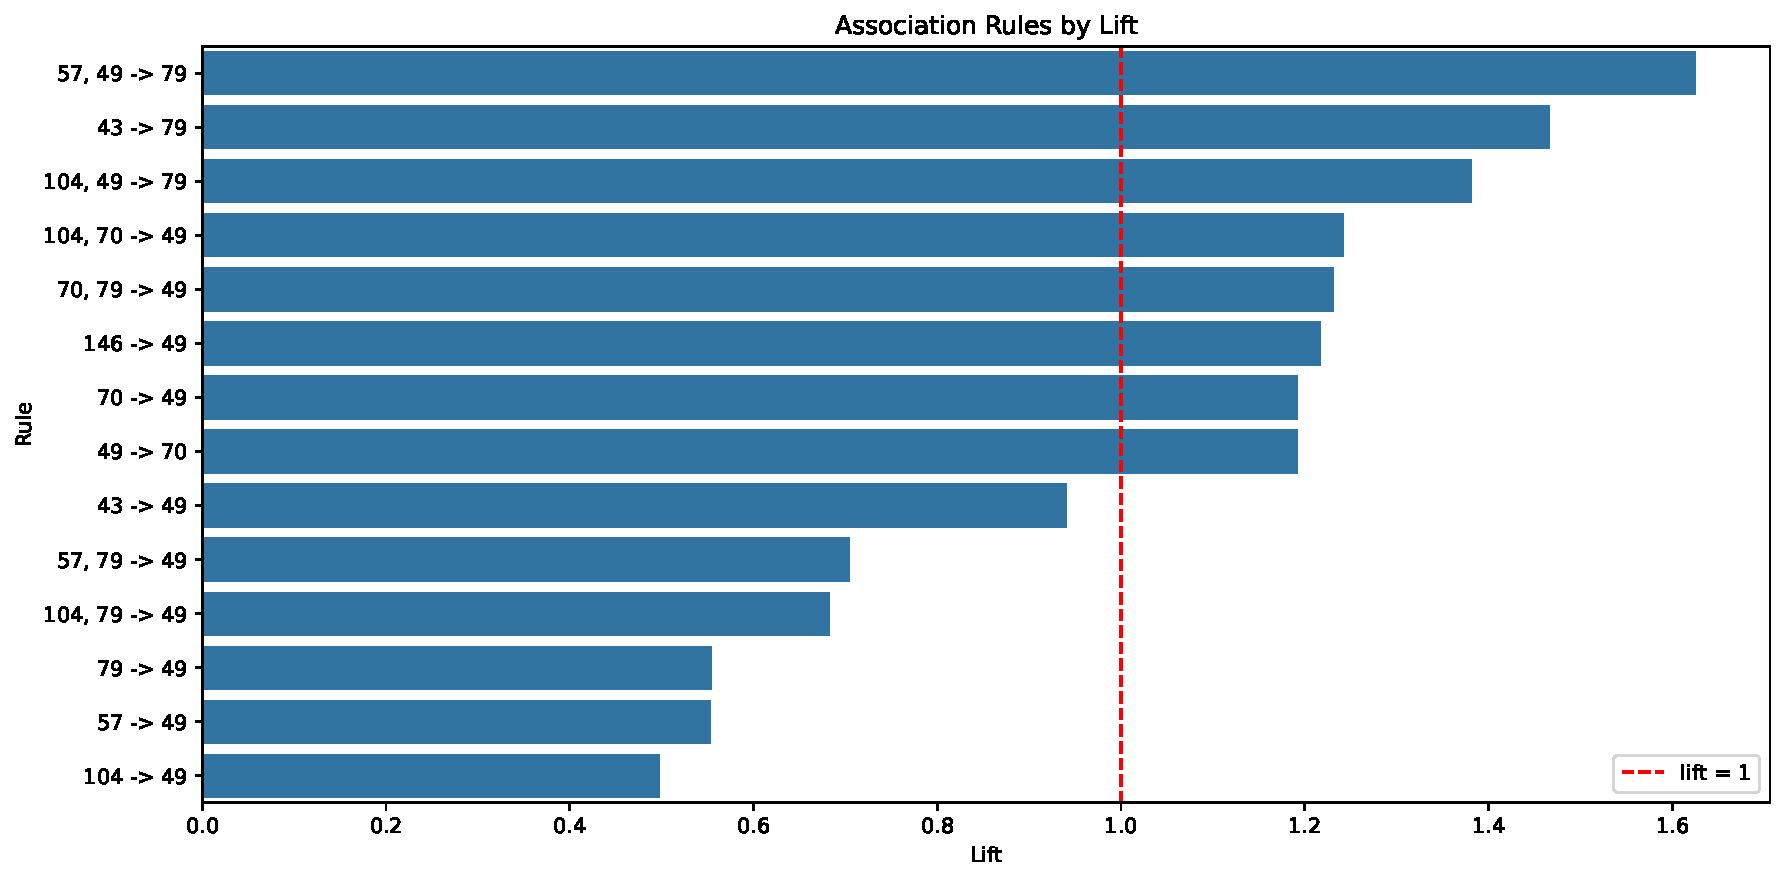
\includegraphics[width=\textwidth]{assets/association_rules_lift.pdf}
    \caption{Association rules ranked by lift, with the red dashed line marking lift = 1 (no association). Rules above the line represent genuine co-occurrence patterns.}
\end{figure}

\subsection{Interpretation}

\paragraph{Meaningful associations (lift $>$ 1):}
\begin{itemize}
    \item Persons who use Orgs 57 and 49 have a \textbf{1.63$\times$} higher-than-chance likelihood of also using Org 79.
    \item Persons using Org 43 have a 1.47$\times$ higher chance of also using Org 79.
    \item Persons using Org 70 are very likely (82.3\% confidence) to also use Org 49, though the lift of 1.19 indicates this is only modestly above baseline.
\end{itemize}

\paragraph{Negative associations (lift $<$ 1):}
\begin{itemize}
    \item Persons using only Org 79, Org 57, or Org 104 are actually \textbf{less} likely than average to also use Org 49, suggesting these orgs serve partially distinct user bases.
\end{itemize}

\paragraph{Main finding.} Org~79 emerges as a genuine ``hub'' in the co-occurrence graph, drawing users from multiple other organizations with statistically meaningful lift. Most rules involving Org~49 show weak associations because its dominance means most users already transact with it by default.

\section{Time-Series Analysis and Forecasting}

\subsection{Daily Time Series Construction}

Transactions were aggregated to daily counts with \texttt{asfreq('D')} to ensure continuous dates (zero-filled for any missing days). The resulting series spans 993 days from April 14, 2022 to December 31, 2024.

\begin{figure}[H]
    \centering
    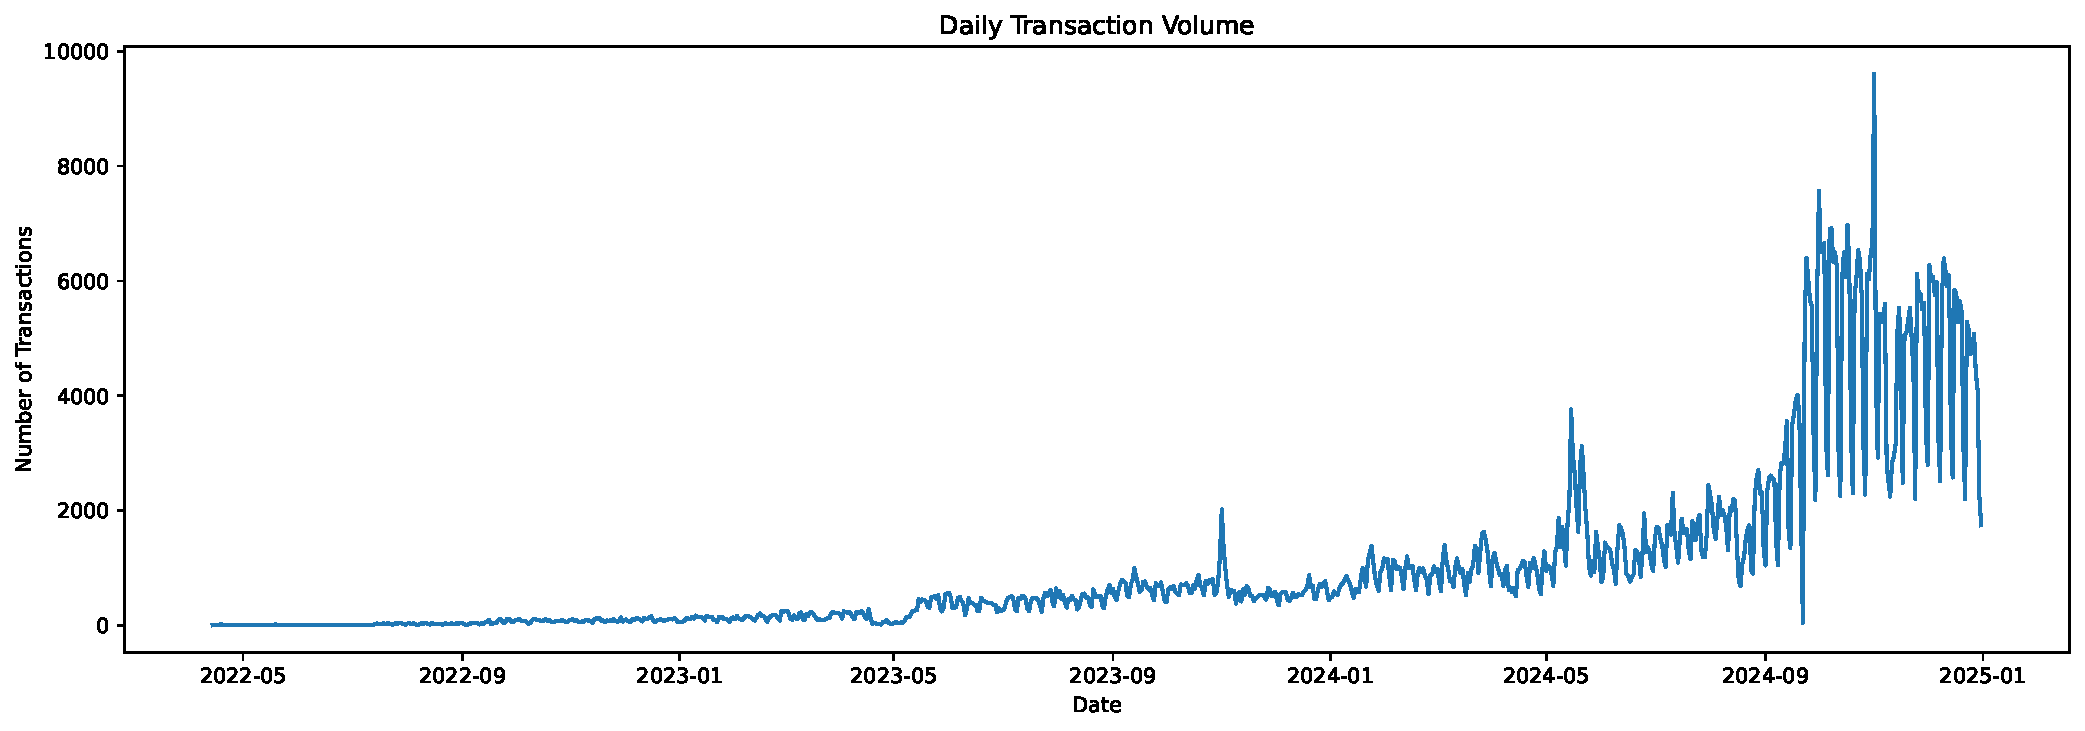
\includegraphics[width=\textwidth]{assets/daily_transaction_volume.pdf}
    \caption{Daily transaction volume from April 2022 to December 2024, showing strong upward trend with growing weekly oscillation and a single-day peak of approximately 9{,}500 transactions in late 2024.}
\end{figure}

Key observations:
\begin{itemize}
    \item Strong upward trend visible across the entire period
    \item Clear weekly oscillation (amplitude growing over time)
    \item Late-2024 volatility including one day peaking at approximately 9{,}500 transactions
\end{itemize}

\subsection{Classical Decomposition}

Using \texttt{seasonal\_decompose} with an additive model and period 7, the series was split into:
\begin{itemize}
    \item \textbf{Trend}: smooth upward curve accelerating after mid-2024
    \item \textbf{Seasonal}: consistent 7-day cycle with amplitude $\approx \pm 400$
    \item \textbf{Residual}: close to 0 for 2022--mid 2024, large and scattered in late 2024
\end{itemize}

\begin{figure}[H]
    \centering
    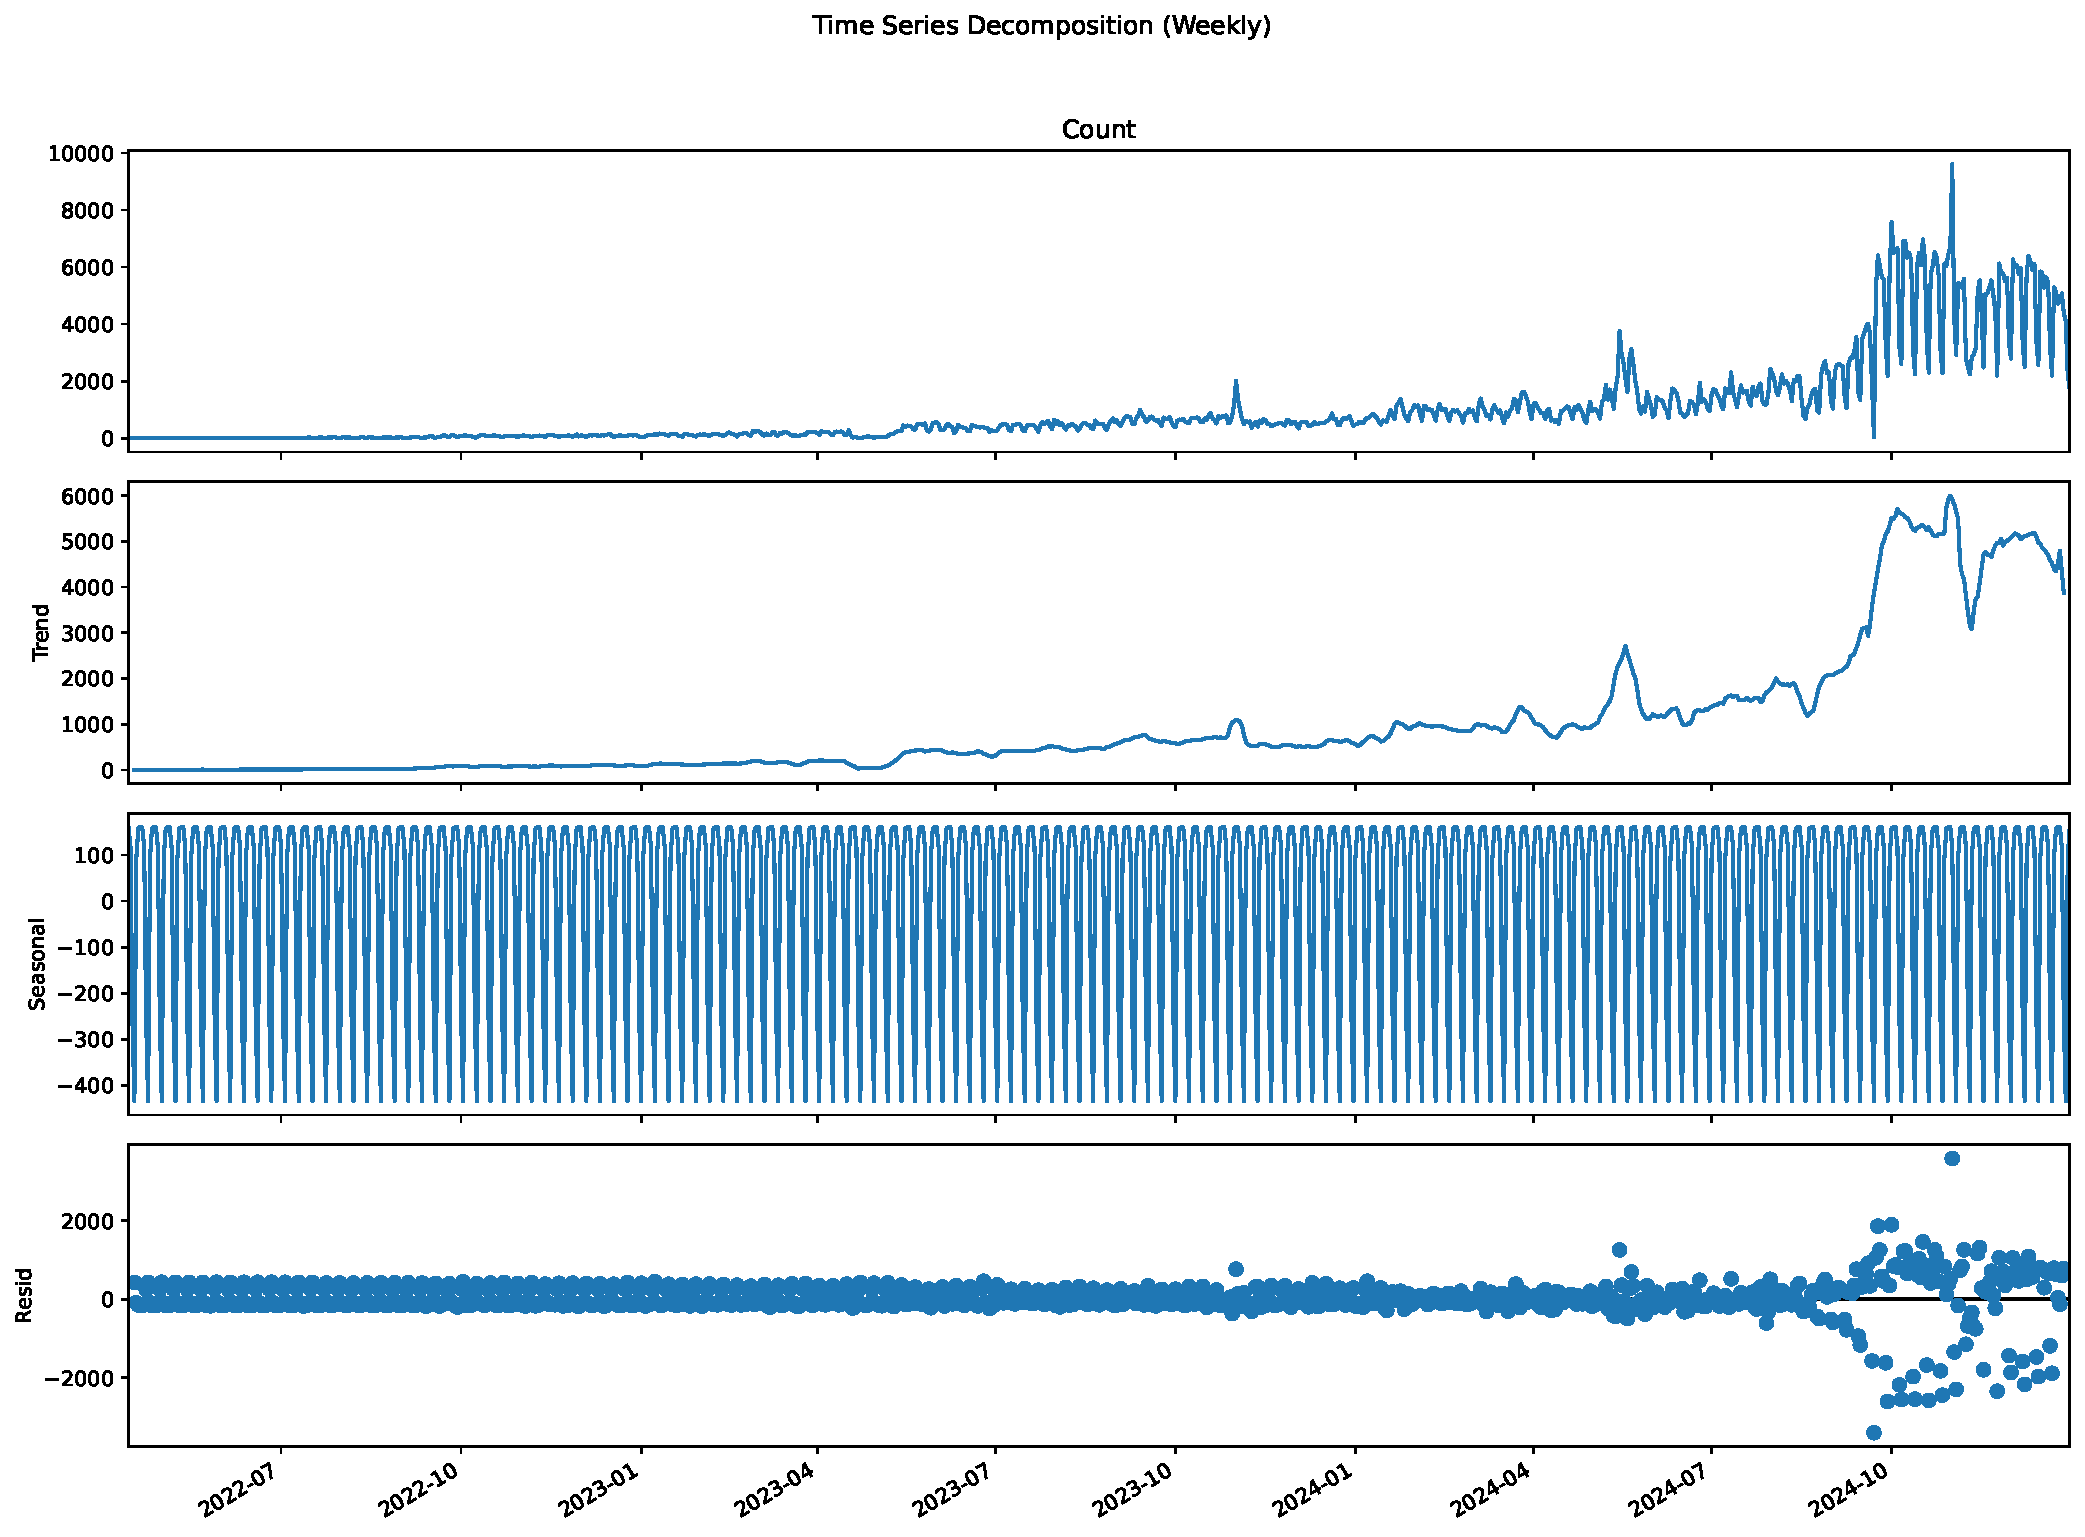
\includegraphics[width=\textwidth]{assets/time_series_decomposition.pdf}
    \caption{Classical additive decomposition of the daily transaction series into trend, seasonal (weekly), and residual components.}
\end{figure}

The growing residuals in late 2024 indicate that trend and seasonality alone cannot fully explain the data in that period, likely driven by Org~49's explosive growth.

\subsection{Stationarity Analysis}

\subsubsection{Augmented Dickey-Fuller Test (Original Series)}

\begin{table}[H]
\centering
\begin{tabular}{ll}
\toprule
\textbf{Statistic} & \textbf{Value} \\
\midrule
ADF Statistic & -1.1162 \\
p-value & 0.7086 \\
Critical Value (1\%) & -3.4371 \\
Critical Value (5\%) & -2.8645 \\
Critical Value (10\%) & -2.5684 \\
\bottomrule
\end{tabular}
\caption{ADF test on original series}
\end{table}

\textbf{Conclusion:} Failed to reject the null hypothesis. The series is \textbf{non-stationary}, as expected from the visible trend.

\subsubsection{ACF and PACF}

\begin{figure}[H]
    \centering
    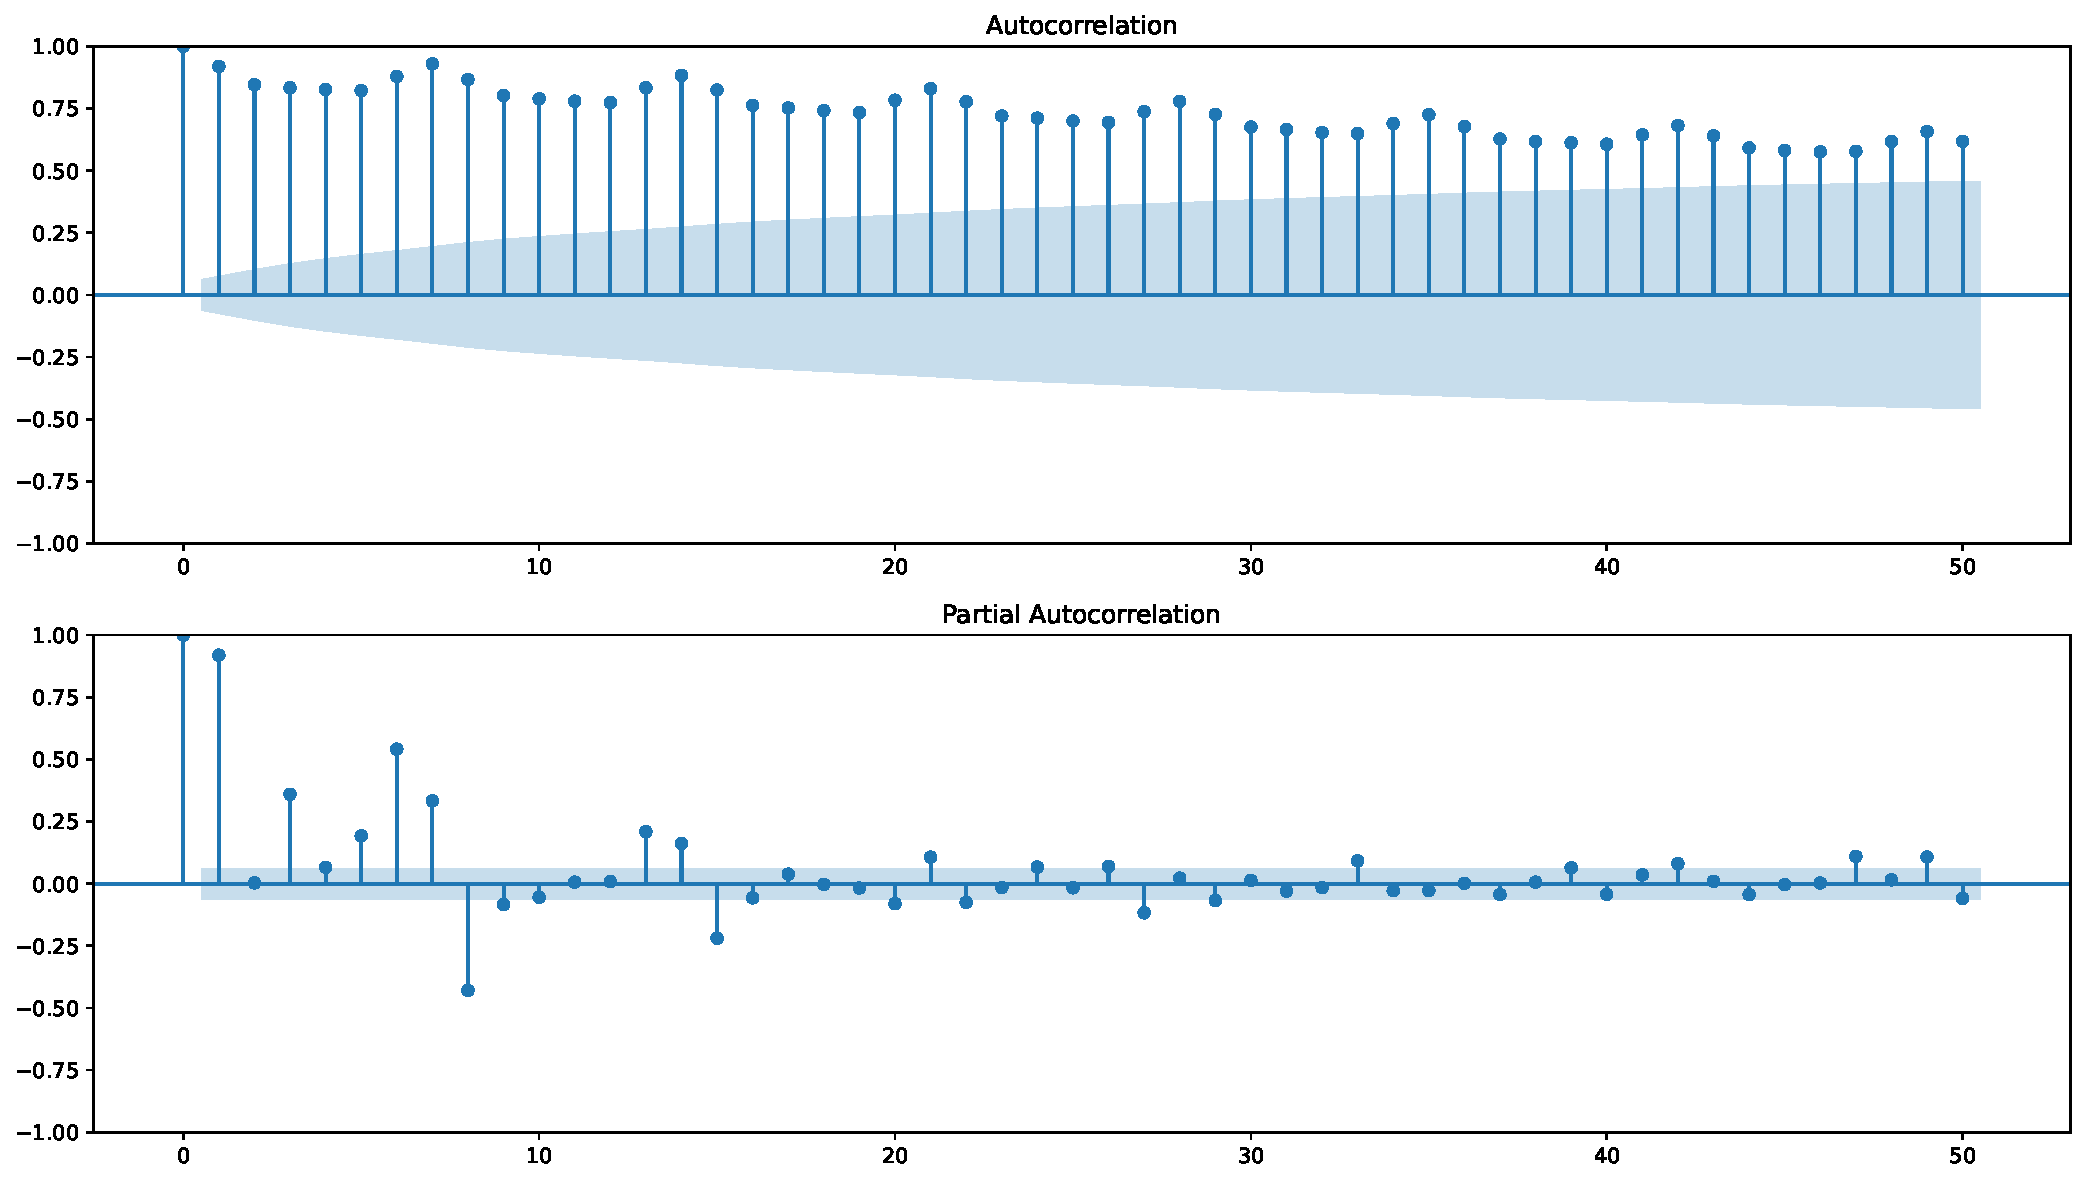
\includegraphics[width=\textwidth]{assets/acf_pacf.pdf}
    \caption{Autocorrelation (ACF) and Partial Autocorrelation (PACF) plots of the daily transaction series. The slow ACF decay confirms non-stationarity; the PACF spike at lag 7 confirms weekly seasonality.}
\end{figure}

\begin{itemize}
    \item \textbf{ACF}: slow decay, all 50 lags significantly correlated, a classic non-stationary signature
    \item \textbf{PACF}: significant spikes at lags 1 ($\approx 0.90$), 2, 7 ($\approx 0.55$), and 8 ($\approx -0.50$)
\end{itemize}

The lag-7 PACF spike strongly confirms weekly seasonality.

\subsubsection{First Differencing}

After applying \texttt{diff()}, the ADF test yielded:
\begin{itemize}
    \item ADF Statistic: -7.2237, p-value: 0.0000
\end{itemize}

The series is stationary in mean, but \textbf{variance grows dramatically in late 2024} (heteroscedasticity), which violates SARIMA's homoscedasticity assumption.

\subsubsection{Log Transformation}

Applying \texttt{np.log1p} before differencing stabilized the variance:
\begin{itemize}
    \item ADF Statistic: -7.1535, p-value: 0.0000
\end{itemize}

\begin{figure}[H]
    \centering
    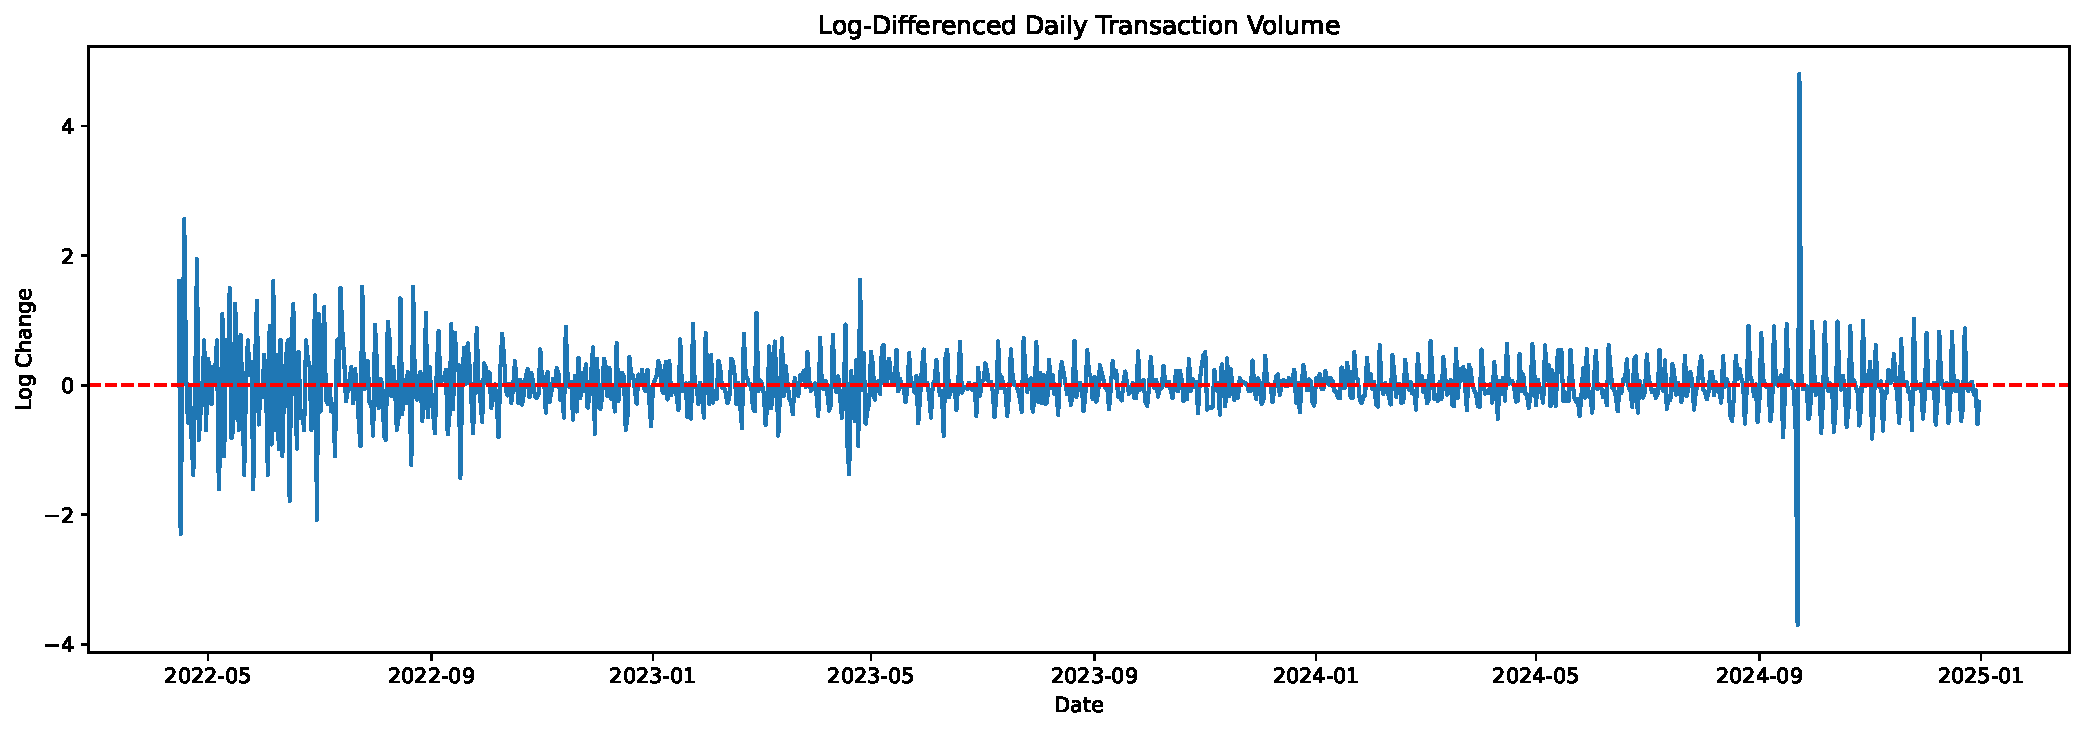
\includegraphics[width=\textwidth]{assets/log_differenced_volume.pdf}
    \caption{Log-differenced daily transaction volume, showing stabilized variance compared to simple differencing, used as the input series for SARIMA modeling.}
\end{figure}

The log-differenced series shows much more uniform variance across the entire period and was used for all subsequent SARIMA modeling.

\subsection{SARIMA Model}

\subsubsection{Parameter Selection}

Parameters were derived from ACF/PACF analysis:
\begin{itemize}
    \item Non-seasonal: $(p, d, q) = (1, 1, 1)$
    \item Seasonal: $(P, D, Q, s) = (1, 1, 1, 7)$
\end{itemize}

The training set comprised 963 days; the test set was the last 30 days (December 2-31, 2024).

\subsubsection{Model Summary}

Key coefficient estimates:

\begin{table}[H]
\centering
\begin{tabular}{lrrr}
\toprule
\textbf{Parameter} & \textbf{Coef} & \textbf{P$>$|z|} & \textbf{Significant?} \\
\midrule
ar.L1 & 0.3626 & 0.000 & Yes \\
ma.L1 & -0.7864 & 0.000 & Yes \\
ar.S.L7 & 0.0359 & 0.170 & No \\
ma.S.L7 & -1.0566 & 0.000 & Yes \\
sigma2 & 0.1086 & 0.000 & Yes \\
\bottomrule
\end{tabular}
\caption{SARIMA(1,1,1)(1,1,1,7) coefficients}
\end{table}

Model diagnostics:
\begin{itemize}
    \item AIC: 714.128, BIC: 738.261
    \item Ljung-Box $p = 0.55$: no residual autocorrelation (good)
    \item Jarque-Bera $p = 0.00$: residuals not normally distributed
    \item Heteroscedasticity $p = 0.00$: variance not constant (expected given late-2024 volatility)
\end{itemize}

\subsubsection{Test Set Forecast}

\begin{figure}[H]
    \centering
    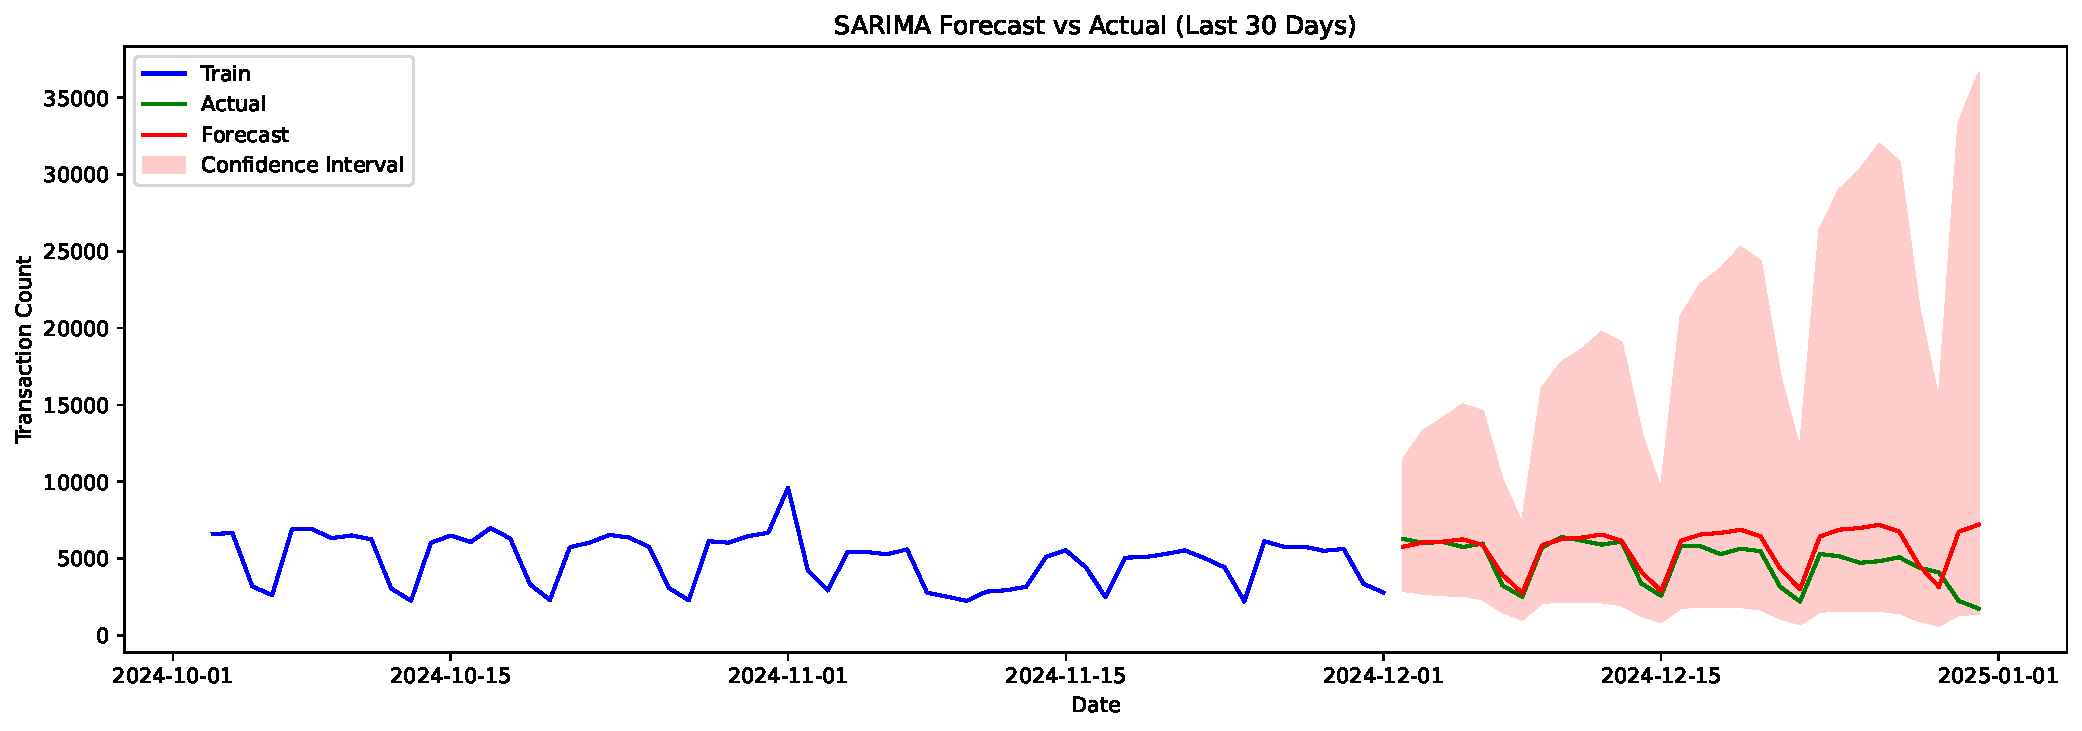
\includegraphics[width=\textwidth]{assets/sarima_forecast.pdf}
    \caption{SARIMA(1,1,1)(1,1,1,7) forecast vs actual transactions for December 2024, with 95\% confidence interval. The forecast captures the weekly pattern but the confidence interval is wide due to late-2024 volatility.}
\end{figure}

SARIMA evaluation metrics:
\begin{itemize}
    \item MAE: 1040.93
    \item RMSE: 1614.83
    \item MAPE: 32.98\%
\end{itemize}

The forecast captures the weekly pattern reasonably well but the confidence interval is very wide in late December due to variance amplification through the log$^{-1}$ transformation.

\subsection{Auto ARIMA}

Using \texttt{pmdarima.auto\_arima} with stepwise search, the best model found was $\text{SARIMAX}(4, 1, 2)(2, 0, [1], 7)$. Despite having more parameters and lower residual autocorrelation (Ljung-Box $p = 0.99$), it performed \textit{worse} on the test set:

\begin{itemize}
    \item MAE: 1207.19
    \item RMSE: 1763.48
    \item MAPE: 36.96\%
\end{itemize}

This illustrates that more complex models are not always better. The manual (1,1,1)(1,1,1,7) choice generalized better despite having lower in-sample fit.

\subsection{Chronos Foundation Model}

The \texttt{chronos-t5-small} pretrained model was used with the following configuration:
\begin{itemize}
    \item Model: \texttt{amazon/chronos-t5-small}
    \item Device: CPU
    \item Prediction length: 30
    \item Samples: 20 (for uncertainty quantification)
\end{itemize}

Chronos requires no stationarity assumption, no manual parameter tuning, and no ACF/PACF analysis. The model was given the raw log-scaled training series as context and asked to forecast 30 days.

\begin{figure}[H]
    \centering
    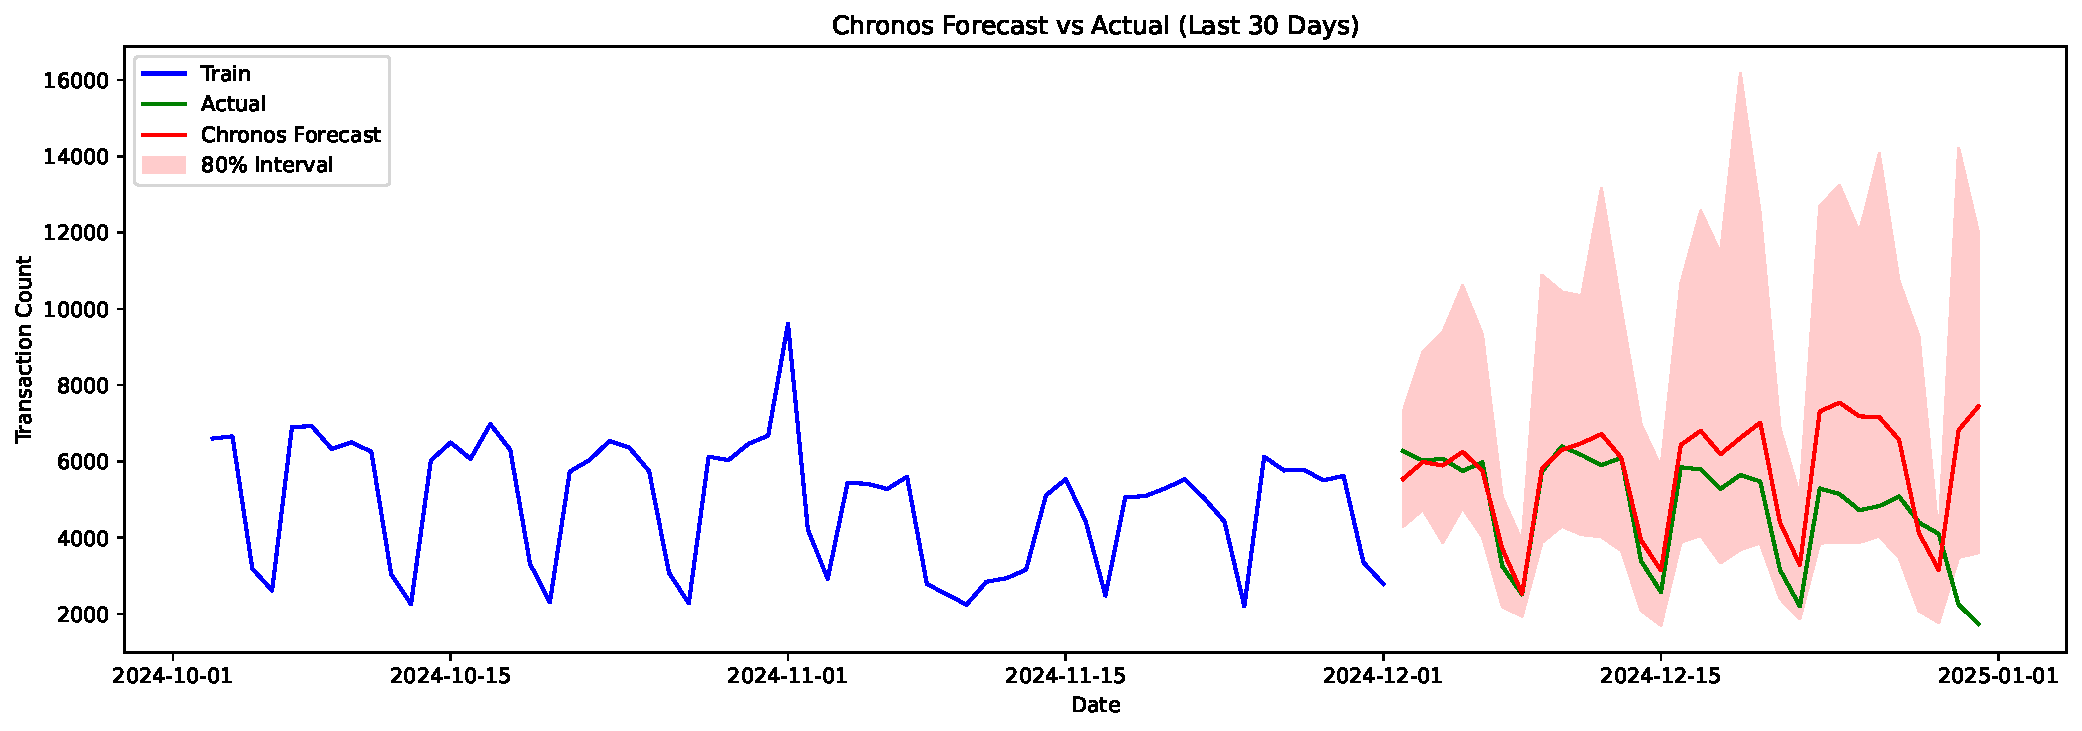
\includegraphics[width=\textwidth]{assets/chronos_forecast.pdf}
    \caption{Chronos foundation model forecast vs actual transactions for December 2024, with 80\% prediction interval. The forecast closely tracks actual values with a tighter uncertainty band than SARIMA.}
\end{figure}

Chronos evaluation metrics:
\begin{itemize}
    \item MAE: 799.36
    \item RMSE: 1266.05
    \item MAPE: 25.15\%
\end{itemize}

\subsection{Model Comparison}

\begin{table}[H]
\centering
\begin{tabular}{lrrr}
\toprule
\textbf{Model} & \textbf{MAE} & \textbf{RMSE} & \textbf{MAPE (\%)} \\
\midrule
Manual SARIMA (1,1,1)(1,1,1,7) & 1040.93 & 1614.83 & 32.98 \\
Auto ARIMA (4,1,2)(2,0,[1],7) & 1207.19 & 1763.48 & 36.96 \\
\textbf{Chronos (chronos-t5-small)} & \textbf{799.36} & \textbf{1266.05} & \textbf{25.15} \\
\bottomrule
\end{tabular}
\caption{Forecast accuracy comparison on 30-day test set}
\end{table}

\begin{figure}[H]
    \centering
    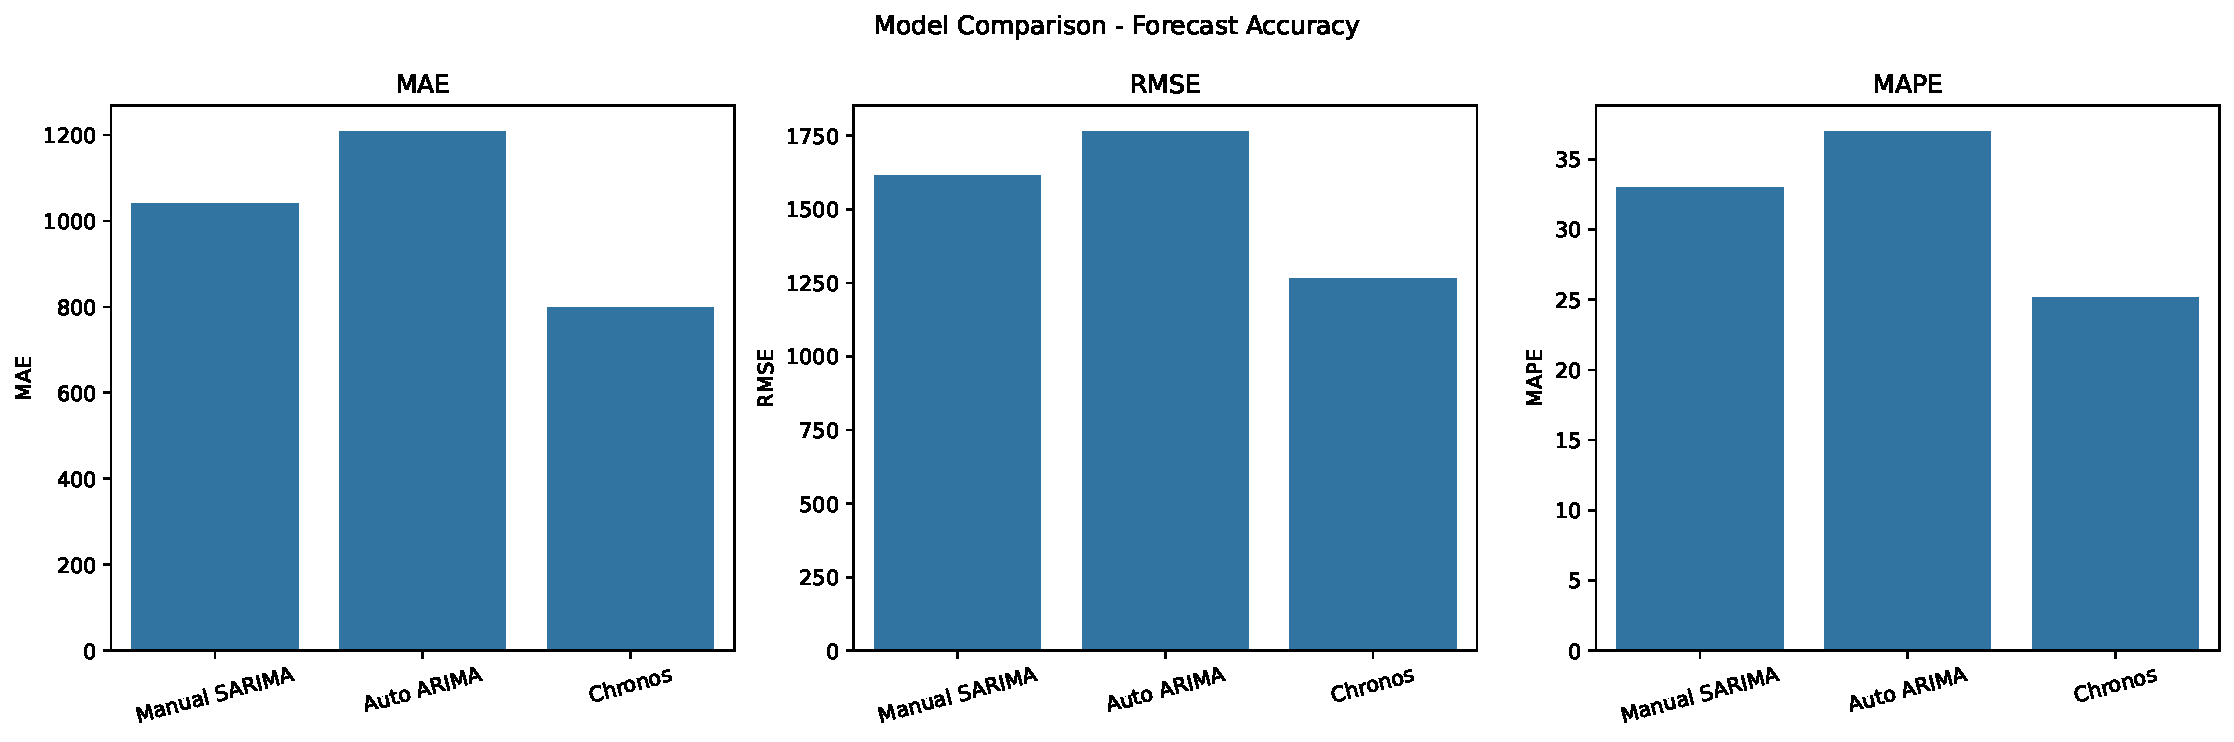
\includegraphics[width=\textwidth]{assets/model_comparison.pdf}
    \caption{Forecast accuracy comparison across all three models on the 30-day test set. Chronos achieves the lowest error on all three metrics.}
\end{figure}

\textbf{Chronos delivered approximately 24\% better MAPE than manual SARIMA and 32\% better than Auto ARIMA with zero tuning.} This demonstrates the practical value of foundation models on non-stationary series with changing variance, exactly the conditions where classical models struggle.

\section{Organization Clustering}

\subsection{Motivation and Features}

With 95 unique organizations, the goal was to identify behaviorally similar groups. Four features were engineered per organization:

\begin{itemize}
    \item \textbf{TotalTransactions}: org's overall activity size
    \item \textbf{RefusalRate}: proportion of refused operations (StatusId = 20)
    \item \textbf{UniquePersons}: number of distinct persons interacting with the org
    \item \textbf{AvgDailyTransactions}: average transactions per active day
\end{itemize}

\texttt{Type1Ratio} and \texttt{CardlessRate} were considered but excluded: the former has no known interpretation, and the latter lacks clear business meaning in this context.

\subsection{Methodology}

\textbf{Hierarchical clustering} with Ward linkage was chosen over K-Means because:
\begin{itemize}
    \item With only 95 data points, hierarchical is fast and produces an informative dendrogram
    \item No need to pre-specify the cluster count
    \item Handles outliers (especially Org 49) more gracefully
\end{itemize}

Features were scaled using \texttt{StandardScaler} because the ranges vary by orders of magnitude (e.g., \texttt{TotalTransactions} from 5 to 620{,}445, while \texttt{RefusalRate} is bounded in $[0, 1]$).

\subsection{Cluster Count Selection}

\begin{figure}[H]
    \centering
    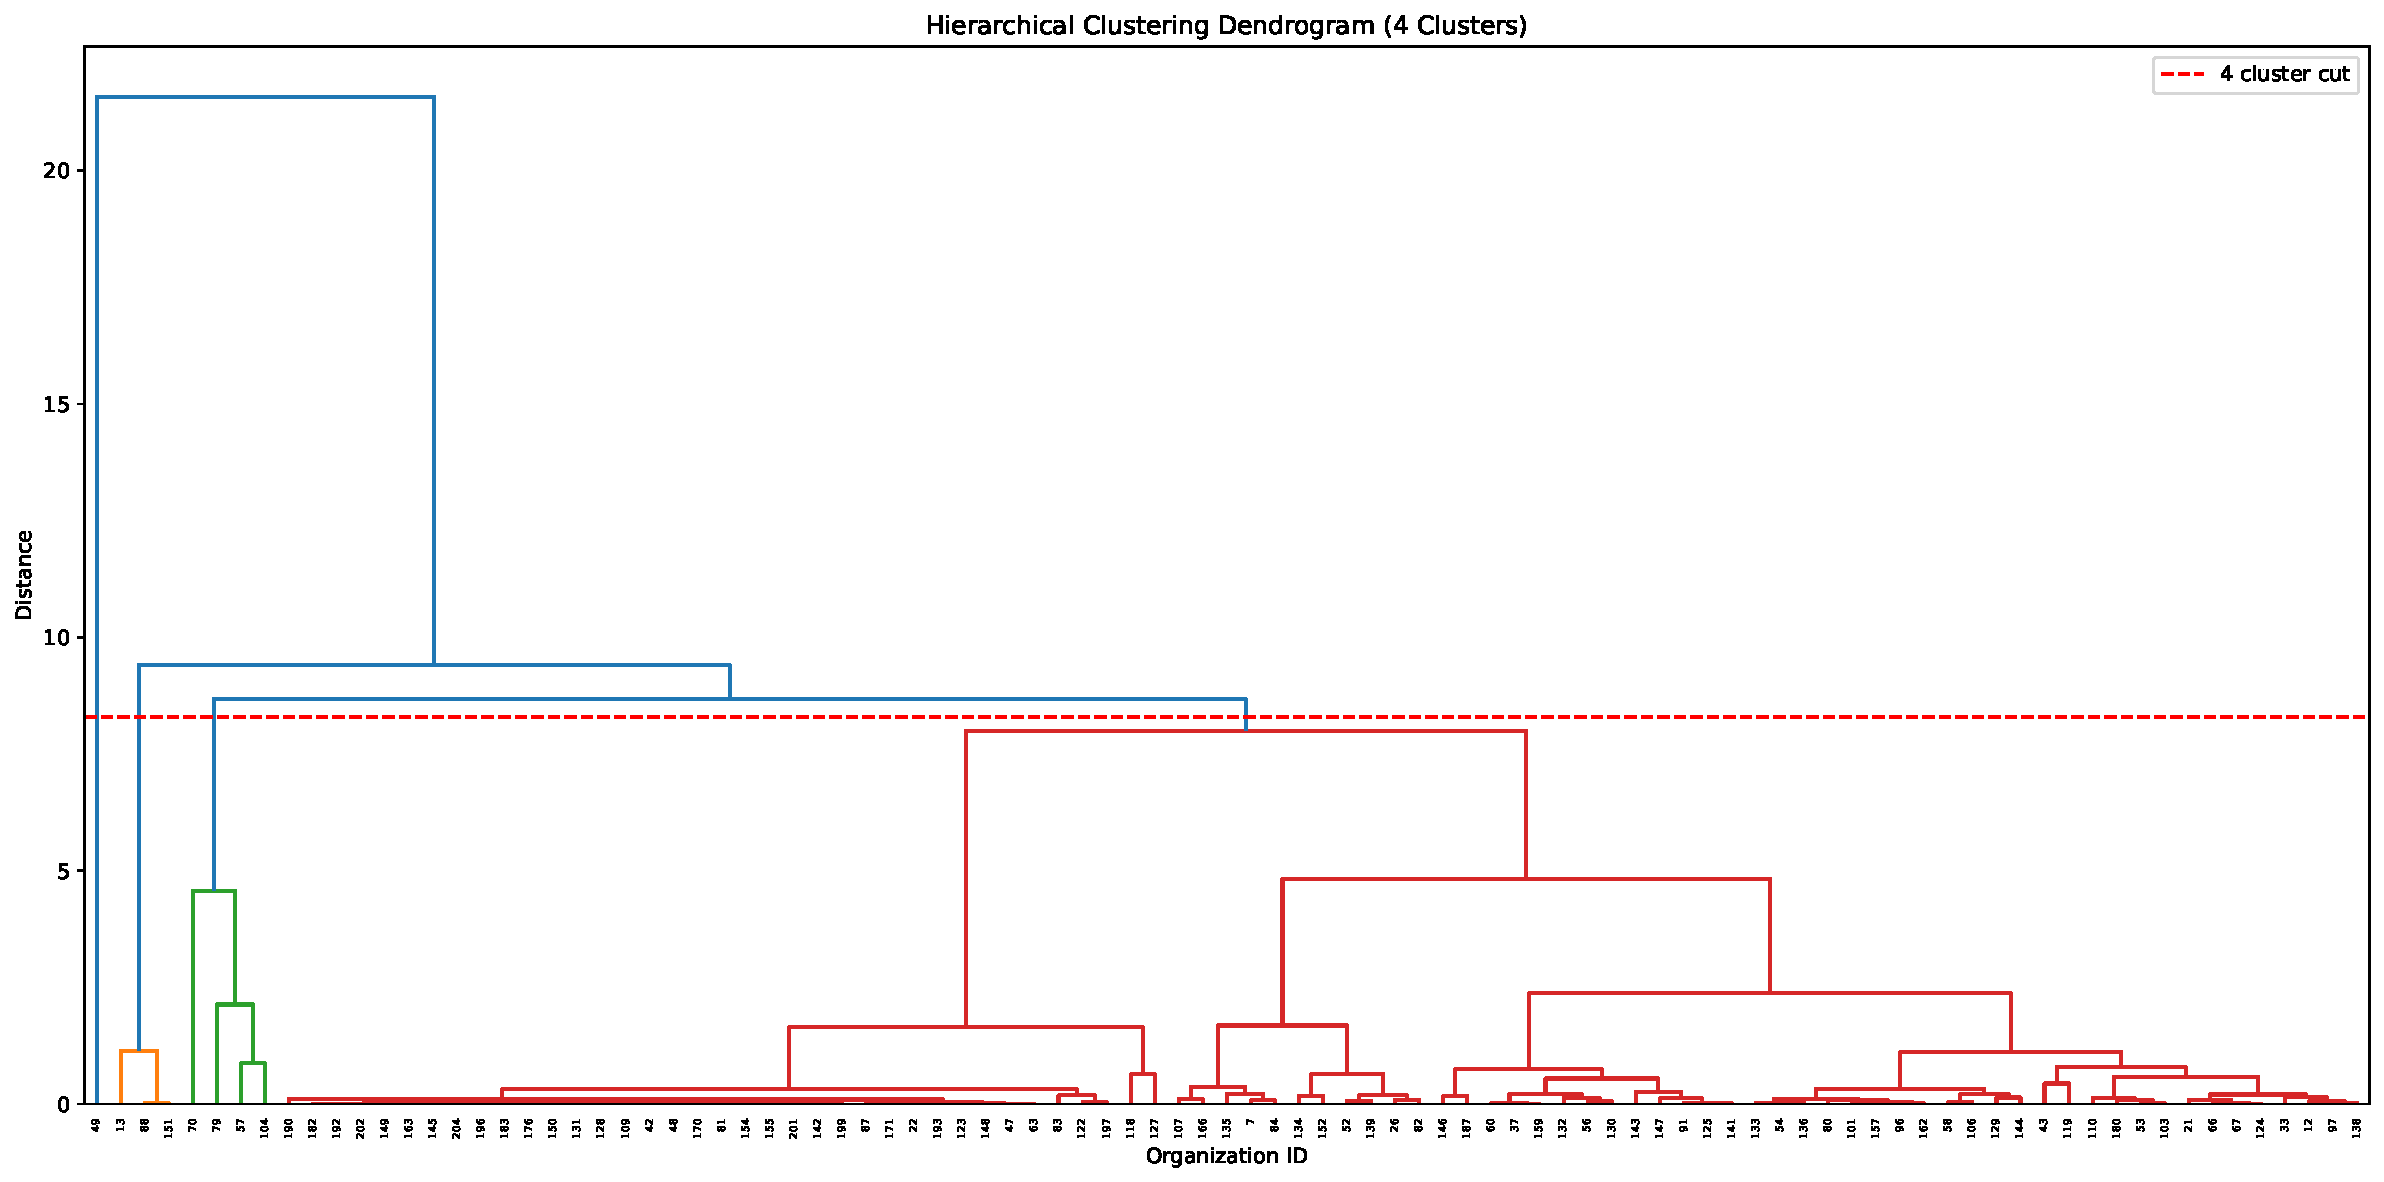
\includegraphics[width=\textwidth]{assets/dendrogram.pdf}
    \caption{Hierarchical clustering dendrogram of 95 organizations using Ward linkage. The red dashed line at distance 8.3 marks the cut point yielding 4 clusters.}
\end{figure}

Cluster validation metrics for different values of $k$:

\begin{table}[H]
\centering
\begin{tabular}{lrrr}
\toprule
\textbf{k} & \textbf{Silhouette} & \textbf{Davies-Bouldin} & \textbf{Calinski-Harabasz} \\
\midrule
3 & 0.702 & 0.228 & 123.6 \\
4 & 0.684 & 0.517 & 145.8 \\
5 & 0.569 & 0.500 & 233.0 \\
\bottomrule
\end{tabular}
\caption{Clustering evaluation metrics}
\end{table}

Although $k=3$ is marginally better by Silhouette and Davies-Bouldin, \textbf{$k=4$ was chosen} based on domain interpretability: at $k=3$ the high-volume organizations (57, 70, 79, 104) are grouped together with all 87 regular orgs, obscuring a genuinely distinct behavioral tier.

\subsection{Cluster Profiles}

\begin{table}[H]
\centering
\begin{tabular}{lrrrr}
\toprule
\textbf{Cluster} & \textbf{Total Tx} & \textbf{Refusal Rate} & \textbf{Unique Persons} & \textbf{Avg Daily} \\
\midrule
Inactive/Problematic & 6.33 & 0.93 & 1.33 & 2.83 \\
High Volume & 67{,}912.75 & 0.23 & 41{,}815.25 & 163.73 \\
Regular & 1{,}240.06 & 0.14 & 388.40 & 6.08 \\
Dominant & 620{,}445.00 & 0.17 & 162{,}649.00 & 699.49 \\
\bottomrule
\end{tabular}
\caption{Mean feature values per cluster}
\end{table}

\begin{figure}[H]
    \centering
    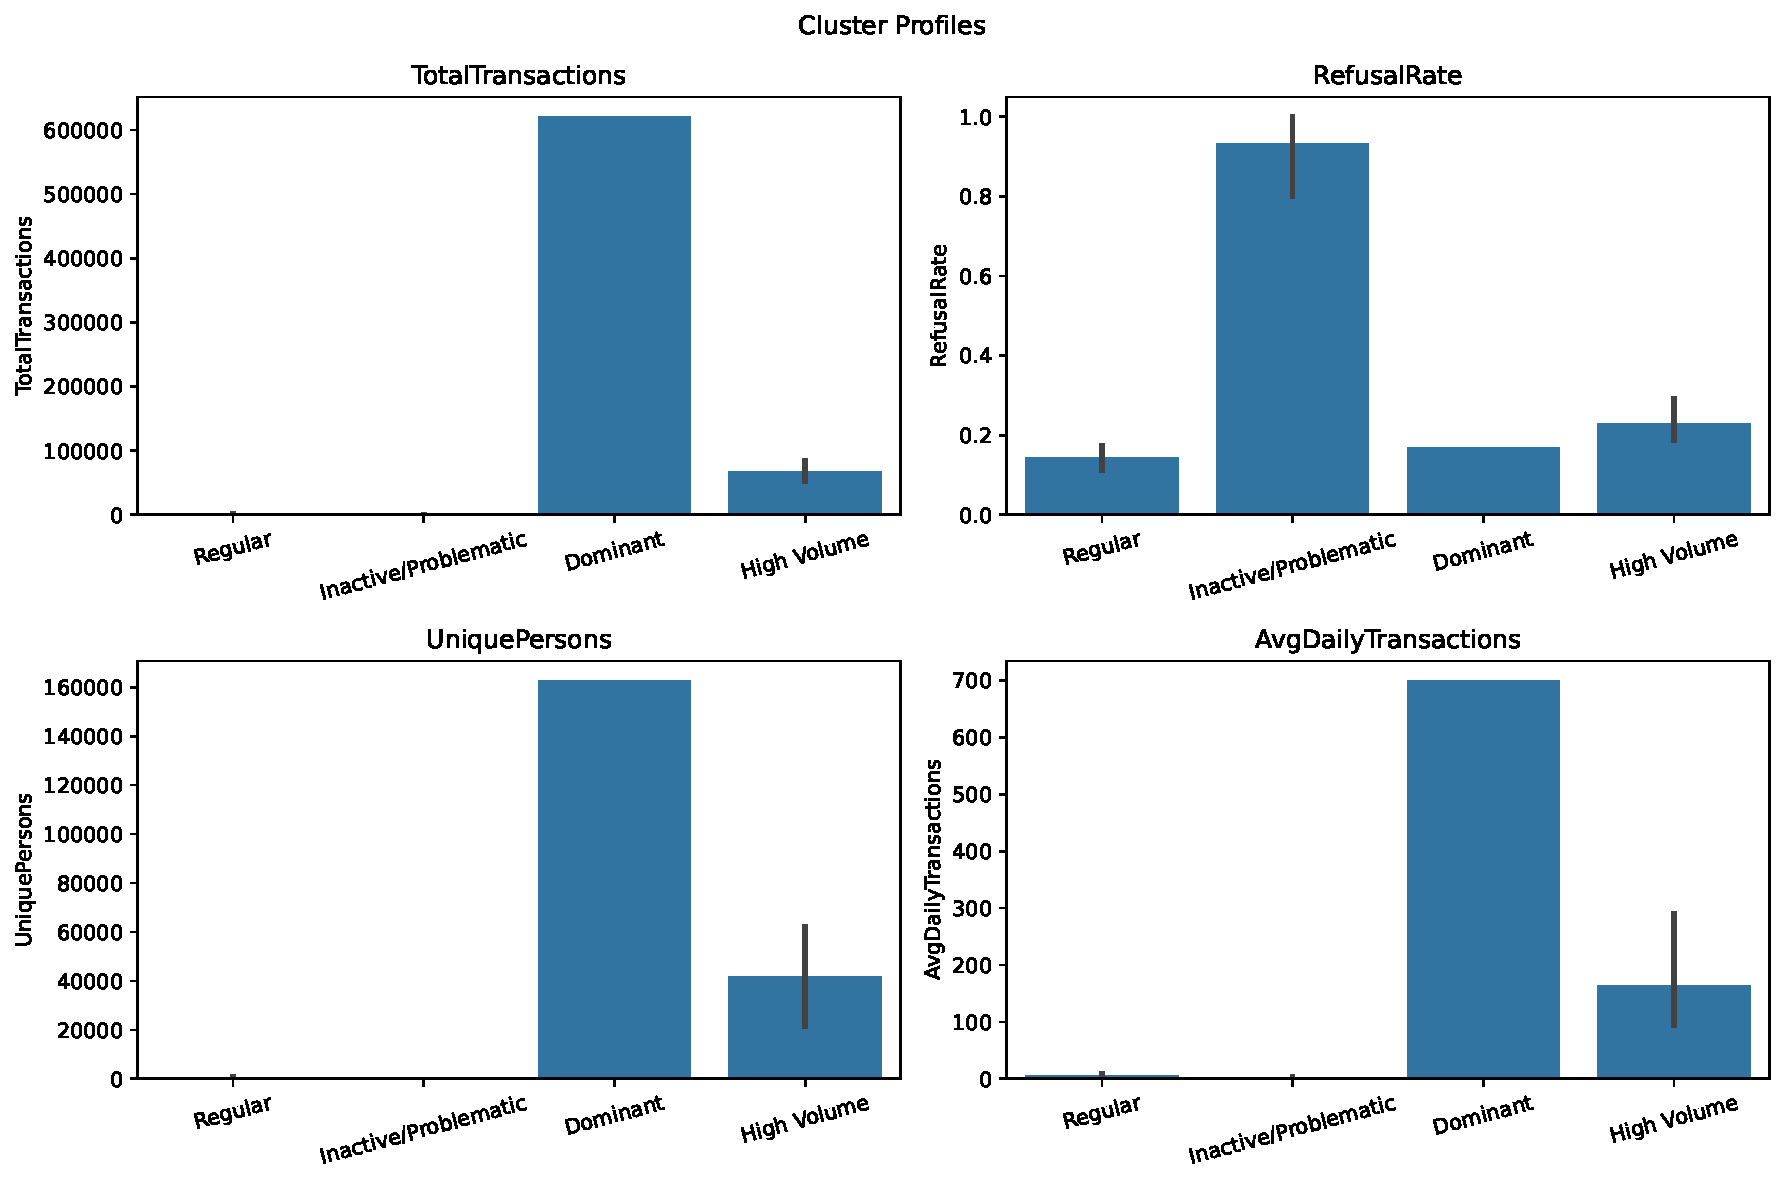
\includegraphics[width=\textwidth]{assets/cluster_profiles.pdf}
    \caption{Mean feature values per cluster across all four dimensions, showing the clear separation between Dominant, High Volume, Regular, and Inactive/Problematic organizations.}
\end{figure}

\subsubsection{Cluster Descriptions}

\paragraph{Dominant (1 org):} \{49\}. A single organization commanding 62\% of all transactions and 69\% of unique users. Forms its own cluster due to its extreme scale.

\paragraph{High Volume (4 orgs):} \{57, 70, 79, 104\}. Mid-to-high volume organizations with the highest refusal rate among active clusters (23\%). These are the "tier 2" orgs that still serve tens of thousands of users each.

\paragraph{Regular (87 orgs):} The bulk of the dataset's organizations. Low-to-medium volume (avg $\approx 1{,}240$ transactions), lowest refusal rate (14\%), moderate reach. These represent the typical organization.

\paragraph{Inactive/Problematic (3 orgs):} \{13, 88, 151\}. All three have nearly zero activity (2-12 transactions total) and 80--100\% refusal rates, each serving only 1-2 persons. These are likely misconfigured, suspended, or abandoned organizations that reject essentially all requests.

\section{Key Findings and Conclusions}

\subsection{Overall Findings}

\begin{enumerate}
    \item \textbf{Extreme concentration.} Org 49 alone accounts for 62\% of transactions and 69\% of unique persons. This organization shapes virtually every aggregate trend observed in the dataset.

    \item \textbf{Strong temporal patterns.} The data exhibits clear weekly seasonality (confirmed by ACF/PACF and decomposition) and an exponential growth trend, particularly after mid-2024.

    \item \textbf{ID column is unreliable.} Transaction IDs are recycled over time with a typical gap of $\sim$240 days between reuses. They cannot serve as unique keys.

    \item \textbf{Most users are one-timers.} 34.8\% of persons have exactly one transaction. The RF analysis's largest segment is "Occasional" (51\% of users), a typical long-tail behavior.

    \item \textbf{Org 79 is a co-occurrence hub.} Among 14 significant association rules, Org 79 receives the most cross-org traffic, with lift values up to 1.63, genuinely beyond chance.

    \item \textbf{Chronos outperforms SARIMA.} On a 30-day test horizon, Chronos achieved MAPE 25.15\% vs 32.98\% for manual SARIMA, without any tuning. Foundation models are a strong default for this kind of non-stationary, volatile series.

    \item \textbf{Four natural org clusters.} Dominant, High Volume, Regular, and Inactive/Problematic. The Inactive/Problematic cluster flags three orgs (13, 88, 151) with 80--100\% refusal rates that may warrant operational review.
\end{enumerate}

\subsection{Limitations}

\begin{itemize}
    \item \textbf{No monetary data.} The dataset contains no transaction value/amount, preventing full RFM analysis and CLV modeling.
    \item \textbf{Unknown transaction type meaning.} TransactionTypeId values (1 and 2) lack documentation; no lookup table is provided.
    \item \textbf{Org 49 dominance.} The heavy concentration in one org biases many analyses. Results often reflect Org 49's behavior more than general system patterns.
    \item \textbf{Late-2024 volatility.} Models trained on stable 2022--mid-2024 data struggle with the rapid growth in late 2024.
    \item \textbf{Data ends December 2024.} Forecast outputs cannot be validated without newer data.
\end{itemize}

\subsection{Recommendations for Future Work}

\begin{itemize}
    \item \textbf{Classification model.} A refusal-prediction binary classifier (features: OrgId, TransactionTypeId, Hour, DayOfWeek, card presence) would be a natural next step.
    \item \textbf{Operational review.} The three Inactive/Problematic orgs (13, 88, 151) should be audited; they may be suspended accounts or misconfigurations.
    \item \textbf{Per-org forecasting.} Separate Chronos models per top org would produce more actionable forecasts than the aggregate series.
    \item \textbf{Org 49 deep-dive.} Given its dominance, analyzing Org 49 as its own dataset could reveal patterns masked by aggregation.
\end{itemize}

\section{Technical Stack}

\begin{table}[H]
\centering
\begin{tabular}{ll}
\toprule
\textbf{Library} & \textbf{Purpose} \\
\midrule
pandas & Data loading and manipulation \\
numpy & Numerical operations \\
matplotlib, seaborn & Visualization \\
scikit-learn & Scaling, clustering metrics \\
scipy & Hierarchical clustering (linkage, dendrogram) \\
statsmodels & SARIMA, decomposition, ADF, ACF/PACF \\
pmdarima & Auto ARIMA \\
mlxtend & FP-Growth, TransactionEncoder, association rules \\
chronos-forecasting & Foundation model time-series forecasting \\
torch & Chronos backend \\
\bottomrule
\end{tabular}
\caption{Key Python libraries used}
\end{table}

\paragraph{Environment.} Python virtual environment with Jupyter kernel connected via VS Code, ensuring reproducibility through notebook-level \texttt{!pip install} cells.

\end{document}
